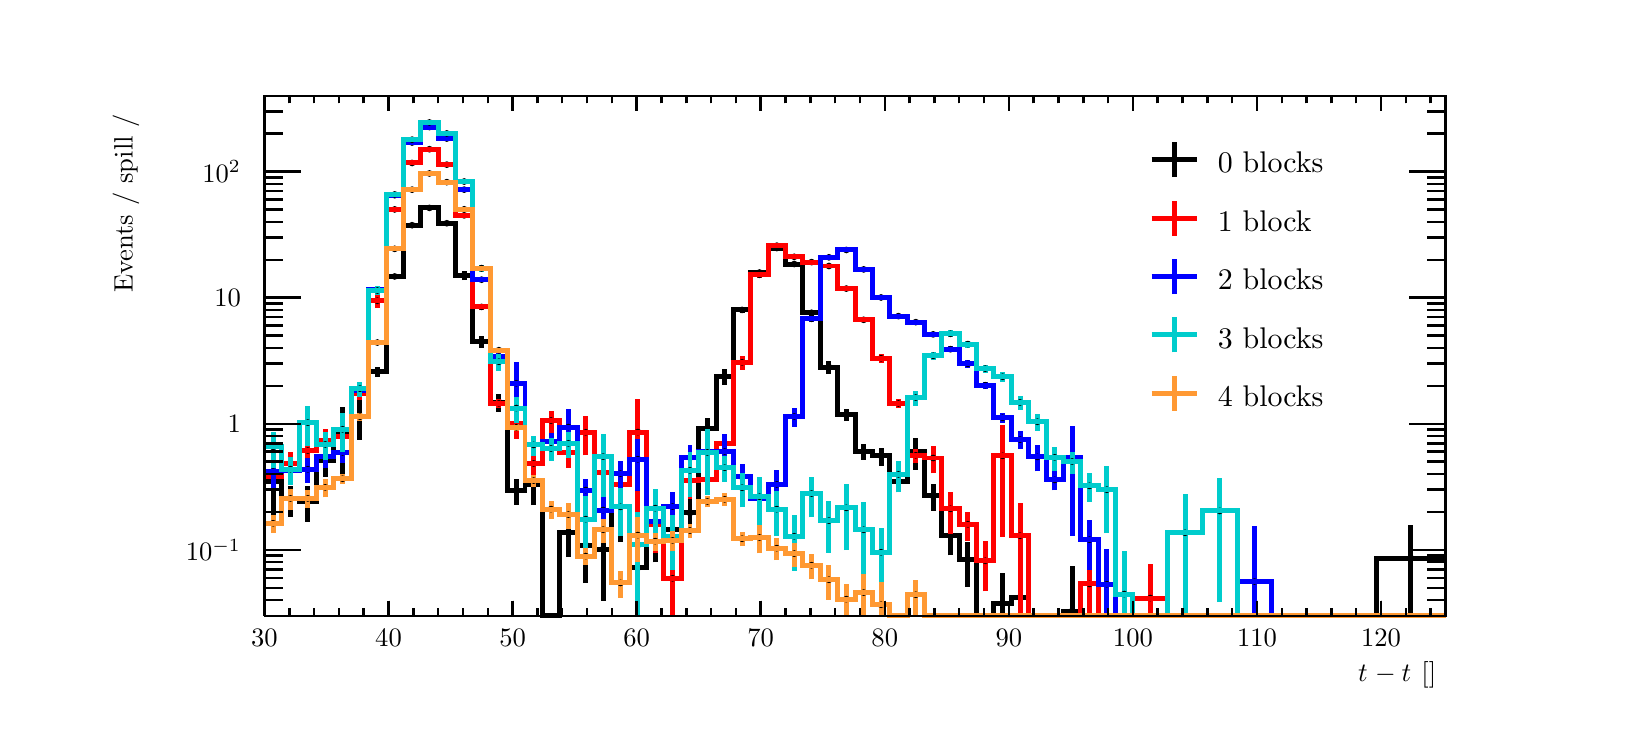
\begin{tikzpicture}
\pgfdeclareplotmark{cross} {
\pgfpathmoveto{\pgfpoint{-0.3\pgfplotmarksize}{\pgfplotmarksize}}
\pgfpathlineto{\pgfpoint{+0.3\pgfplotmarksize}{\pgfplotmarksize}}
\pgfpathlineto{\pgfpoint{+0.3\pgfplotmarksize}{0.3\pgfplotmarksize}}
\pgfpathlineto{\pgfpoint{+1\pgfplotmarksize}{0.3\pgfplotmarksize}}
\pgfpathlineto{\pgfpoint{+1\pgfplotmarksize}{-0.3\pgfplotmarksize}}
\pgfpathlineto{\pgfpoint{+0.3\pgfplotmarksize}{-0.3\pgfplotmarksize}}
\pgfpathlineto{\pgfpoint{+0.3\pgfplotmarksize}{-1.\pgfplotmarksize}}
\pgfpathlineto{\pgfpoint{-0.3\pgfplotmarksize}{-1.\pgfplotmarksize}}
\pgfpathlineto{\pgfpoint{-0.3\pgfplotmarksize}{-0.3\pgfplotmarksize}}
\pgfpathlineto{\pgfpoint{-1.\pgfplotmarksize}{-0.3\pgfplotmarksize}}
\pgfpathlineto{\pgfpoint{-1.\pgfplotmarksize}{0.3\pgfplotmarksize}}
\pgfpathlineto{\pgfpoint{-0.3\pgfplotmarksize}{0.3\pgfplotmarksize}}
\pgfpathclose
\pgfusepathqstroke
}
\pgfdeclareplotmark{cross*} {
\pgfpathmoveto{\pgfpoint{-0.3\pgfplotmarksize}{\pgfplotmarksize}}
\pgfpathlineto{\pgfpoint{+0.3\pgfplotmarksize}{\pgfplotmarksize}}
\pgfpathlineto{\pgfpoint{+0.3\pgfplotmarksize}{0.3\pgfplotmarksize}}
\pgfpathlineto{\pgfpoint{+1\pgfplotmarksize}{0.3\pgfplotmarksize}}
\pgfpathlineto{\pgfpoint{+1\pgfplotmarksize}{-0.3\pgfplotmarksize}}
\pgfpathlineto{\pgfpoint{+0.3\pgfplotmarksize}{-0.3\pgfplotmarksize}}
\pgfpathlineto{\pgfpoint{+0.3\pgfplotmarksize}{-1.\pgfplotmarksize}}
\pgfpathlineto{\pgfpoint{-0.3\pgfplotmarksize}{-1.\pgfplotmarksize}}
\pgfpathlineto{\pgfpoint{-0.3\pgfplotmarksize}{-0.3\pgfplotmarksize}}
\pgfpathlineto{\pgfpoint{-1.\pgfplotmarksize}{-0.3\pgfplotmarksize}}
\pgfpathlineto{\pgfpoint{-1.\pgfplotmarksize}{0.3\pgfplotmarksize}}
\pgfpathlineto{\pgfpoint{-0.3\pgfplotmarksize}{0.3\pgfplotmarksize}}
\pgfpathclose
\pgfusepathqfillstroke
}
\pgfdeclareplotmark{newstar} {
\pgfpathmoveto{\pgfqpoint{0pt}{\pgfplotmarksize}}
\pgfpathlineto{\pgfqpointpolar{44}{0.5\pgfplotmarksize}}
\pgfpathlineto{\pgfqpointpolar{18}{\pgfplotmarksize}}
\pgfpathlineto{\pgfqpointpolar{-20}{0.5\pgfplotmarksize}}
\pgfpathlineto{\pgfqpointpolar{-54}{\pgfplotmarksize}}
\pgfpathlineto{\pgfqpointpolar{-90}{0.5\pgfplotmarksize}}
\pgfpathlineto{\pgfqpointpolar{234}{\pgfplotmarksize}}
\pgfpathlineto{\pgfqpointpolar{198}{0.5\pgfplotmarksize}}
\pgfpathlineto{\pgfqpointpolar{162}{\pgfplotmarksize}}
\pgfpathlineto{\pgfqpointpolar{134}{0.5\pgfplotmarksize}}
\pgfpathclose
\pgfusepathqstroke
}
\pgfdeclareplotmark{newstar*} {
\pgfpathmoveto{\pgfqpoint{0pt}{\pgfplotmarksize}}
\pgfpathlineto{\pgfqpointpolar{44}{0.5\pgfplotmarksize}}
\pgfpathlineto{\pgfqpointpolar{18}{\pgfplotmarksize}}
\pgfpathlineto{\pgfqpointpolar{-20}{0.5\pgfplotmarksize}}
\pgfpathlineto{\pgfqpointpolar{-54}{\pgfplotmarksize}}
\pgfpathlineto{\pgfqpointpolar{-90}{0.5\pgfplotmarksize}}
\pgfpathlineto{\pgfqpointpolar{234}{\pgfplotmarksize}}
\pgfpathlineto{\pgfqpointpolar{198}{0.5\pgfplotmarksize}}
\pgfpathlineto{\pgfqpointpolar{162}{\pgfplotmarksize}}
\pgfpathlineto{\pgfqpointpolar{134}{0.5\pgfplotmarksize}}
\pgfpathclose
\pgfusepathqfillstroke
}
\definecolor{c}{rgb}{1,1,1};
\draw [color=c, fill=c] (0,0) rectangle (20,8.57658);
\draw [color=c, fill=c] (3,1.11495) rectangle (18,7.71892);
\definecolor{c}{rgb}{0,0,0};
\draw [c,line width=0.9] (3,1.11495) -- (3,7.71892) -- (18,7.71892) -- (18,1.11495) -- (3,1.11495);
\definecolor{c}{rgb}{1,1,1};
\draw [color=c, fill=c] (3,1.11495) rectangle (18,7.71892);
\definecolor{c}{rgb}{0,0,0};
\draw [c,line width=0.9] (3,1.11495) -- (3,7.71892) -- (18,7.71892) -- (18,1.11495) -- (3,1.11495);
\draw [c,line width=0.9] (3,1.11495) -- (3.22059,1.11495) -- (3.22059,1.11495) -- (3.44118,1.11495) -- (3.44118,1.11495) -- (3.66176,1.11495) -- (3.66176,1.11495) -- (3.88235,1.11495) -- (3.88235,1.11495) -- (4.10294,1.11495) -- (4.10294,1.11495) --
 (4.32353,1.11495) -- (4.32353,1.11495) -- (4.54412,1.11495) -- (4.54412,1.11495) -- (4.76471,1.11495) -- (4.76471,1.11495) -- (4.98529,1.11495) -- (4.98529,1.11495) -- (5.20588,1.11495) -- (5.20588,1.11495) -- (5.42647,1.11495) -- (5.42647,1.11495)
 -- (5.64706,1.11495) -- (5.64706,1.11495) -- (5.86765,1.11495) -- (5.86765,1.11495) -- (6.08824,1.11495) -- (6.08824,1.11495) -- (6.30882,1.11495) -- (6.30882,1.11495) -- (6.52941,1.11495) -- (6.52941,1.11495) -- (6.75,1.11495) -- (6.75,1.11495) --
 (6.97059,1.11495) -- (6.97059,1.11495) -- (7.19118,1.11495) -- (7.19118,1.11495) -- (7.41176,1.11495) -- (7.41176,1.11495) -- (7.63235,1.11495) -- (7.63235,1.11495) -- (7.85294,1.11495) -- (7.85294,1.11495) -- (8.07353,1.11495) -- (8.07353,1.11495)
 -- (8.29412,1.11495) -- (8.29412,1.11495) -- (8.51471,1.11495) -- (8.51471,1.11495) -- (8.73529,1.11495) -- (8.73529,1.11495) -- (8.95588,1.11495) -- (8.95588,1.11495) -- (9.17647,1.11495) -- (9.17647,1.11495) -- (9.39706,1.11495) --
 (9.39706,1.11495) -- (9.61765,1.11495) -- (9.61765,1.11495) -- (9.83823,1.11495) -- (9.83823,1.11495) -- (10.0588,1.11495) -- (10.0588,1.11495) -- (10.2794,1.11495) -- (10.2794,1.11495) -- (10.5,1.11495) -- (10.5,1.11495) -- (10.7206,1.11495) --
 (10.7206,1.11495) -- (10.9412,1.11495) -- (10.9412,1.11495) -- (11.1618,1.11495) -- (11.1618,1.11495) -- (11.3824,1.11495) -- (11.3824,1.11495) -- (11.6029,1.11495) -- (11.6029,1.11495) -- (11.8235,1.11495) -- (11.8235,1.11495) -- (12.0441,1.11495)
 -- (12.0441,1.11495) -- (12.2647,1.11495) -- (12.2647,1.11495) -- (12.4853,1.11495) -- (12.4853,1.11495) -- (12.7059,1.11495) -- (12.7059,1.11495) -- (12.9265,1.11495) -- (12.9265,1.11495) -- (13.1471,1.11495) -- (13.1471,1.11495) --
 (13.3676,1.11495) -- (13.3676,1.11495) -- (13.5882,1.11495) -- (13.5882,1.11495) -- (13.8088,1.11495) -- (13.8088,1.11495) -- (14.0294,1.11495) -- (14.0294,1.11495) -- (14.4706,1.11495) -- (14.4706,1.11495) -- (14.9118,1.11495) -- (14.9118,1.11495)
 -- (15.3529,1.11495) -- (15.3529,1.11495) -- (15.7941,1.11495) -- (15.7941,1.11495) -- (16.2353,1.11495) -- (16.2353,1.11495) -- (17.1176,1.11495) -- (17.1176,1.11495) -- (18,1.11495);
\draw [c,line width=0.9] (3,1.11495) -- (18,1.11495);
\draw [c,line width=0.9] (3,1.30793) -- (3,1.11495);
\draw [c,line width=0.9] (3.31513,1.21144) -- (3.31513,1.11495);
\draw [c,line width=0.9] (3.63025,1.21144) -- (3.63025,1.11495);
\draw [c,line width=0.9] (3.94538,1.21144) -- (3.94538,1.11495);
\draw [c,line width=0.9] (4.2605,1.21144) -- (4.2605,1.11495);
\draw [c,line width=0.9] (4.57563,1.30793) -- (4.57563,1.11495);
\draw [c,line width=0.9] (4.89076,1.21144) -- (4.89076,1.11495);
\draw [c,line width=0.9] (5.20588,1.21144) -- (5.20588,1.11495);
\draw [c,line width=0.9] (5.52101,1.21144) -- (5.52101,1.11495);
\draw [c,line width=0.9] (5.83613,1.21144) -- (5.83613,1.11495);
\draw [c,line width=0.9] (6.15126,1.30793) -- (6.15126,1.11495);
\draw [c,line width=0.9] (6.46639,1.21144) -- (6.46639,1.11495);
\draw [c,line width=0.9] (6.78151,1.21144) -- (6.78151,1.11495);
\draw [c,line width=0.9] (7.09664,1.21144) -- (7.09664,1.11495);
\draw [c,line width=0.9] (7.41176,1.21144) -- (7.41176,1.11495);
\draw [c,line width=0.9] (7.72689,1.30793) -- (7.72689,1.11495);
\draw [c,line width=0.9] (8.04202,1.21144) -- (8.04202,1.11495);
\draw [c,line width=0.9] (8.35714,1.21144) -- (8.35714,1.11495);
\draw [c,line width=0.9] (8.67227,1.21144) -- (8.67227,1.11495);
\draw [c,line width=0.9] (8.9874,1.21144) -- (8.9874,1.11495);
\draw [c,line width=0.9] (9.30252,1.30793) -- (9.30252,1.11495);
\draw [c,line width=0.9] (9.61765,1.21144) -- (9.61765,1.11495);
\draw [c,line width=0.9] (9.93277,1.21144) -- (9.93277,1.11495);
\draw [c,line width=0.9] (10.2479,1.21144) -- (10.2479,1.11495);
\draw [c,line width=0.9] (10.563,1.21144) -- (10.563,1.11495);
\draw [c,line width=0.9] (10.8782,1.30793) -- (10.8782,1.11495);
\draw [c,line width=0.9] (11.1933,1.21144) -- (11.1933,1.11495);
\draw [c,line width=0.9] (11.5084,1.21144) -- (11.5084,1.11495);
\draw [c,line width=0.9] (11.8235,1.21144) -- (11.8235,1.11495);
\draw [c,line width=0.9] (12.1387,1.21144) -- (12.1387,1.11495);
\draw [c,line width=0.9] (12.4538,1.30793) -- (12.4538,1.11495);
\draw [c,line width=0.9] (12.7689,1.21144) -- (12.7689,1.11495);
\draw [c,line width=0.9] (13.084,1.21144) -- (13.084,1.11495);
\draw [c,line width=0.9] (13.3992,1.21144) -- (13.3992,1.11495);
\draw [c,line width=0.9] (13.7143,1.21144) -- (13.7143,1.11495);
\draw [c,line width=0.9] (14.0294,1.30793) -- (14.0294,1.11495);
\draw [c,line width=0.9] (14.3445,1.21144) -- (14.3445,1.11495);
\draw [c,line width=0.9] (14.6597,1.21144) -- (14.6597,1.11495);
\draw [c,line width=0.9] (14.9748,1.21144) -- (14.9748,1.11495);
\draw [c,line width=0.9] (15.2899,1.21144) -- (15.2899,1.11495);
\draw [c,line width=0.9] (15.605,1.30793) -- (15.605,1.11495);
\draw [c,line width=0.9] (15.9202,1.21144) -- (15.9202,1.11495);
\draw [c,line width=0.9] (16.2353,1.21144) -- (16.2353,1.11495);
\draw [c,line width=0.9] (16.5504,1.21144) -- (16.5504,1.11495);
\draw [c,line width=0.9] (16.8655,1.21144) -- (16.8655,1.11495);
\draw [c,line width=0.9] (17.1807,1.30793) -- (17.1807,1.11495);
\draw [c,line width=0.9] (17.1807,1.30793) -- (17.1807,1.11495);
\draw [c,line width=0.9] (17.4958,1.21144) -- (17.4958,1.11495);
\draw [c,line width=0.9] (17.8109,1.21144) -- (17.8109,1.11495);
\draw [anchor=base] (3,0.729009) node[scale=0.960419, color=c, rotate=0]{30};
\draw [anchor=base] (4.57563,0.729009) node[scale=0.960419, color=c, rotate=0]{40};
\draw [anchor=base] (6.15126,0.729009) node[scale=0.960419, color=c, rotate=0]{50};
\draw [anchor=base] (7.72689,0.729009) node[scale=0.960419, color=c, rotate=0]{60};
\draw [anchor=base] (9.30252,0.729009) node[scale=0.960419, color=c, rotate=0]{70};
\draw [anchor=base] (10.8782,0.729009) node[scale=0.960419, color=c, rotate=0]{80};
\draw [anchor=base] (12.4538,0.729009) node[scale=0.960419, color=c, rotate=0]{90};
\draw [anchor=base] (14.0294,0.729009) node[scale=0.960419, color=c, rotate=0]{100};
\draw [anchor=base] (15.605,0.729009) node[scale=0.960419, color=c, rotate=0]{110};
\draw [anchor=base] (17.1807,0.729009) node[scale=0.960419, color=c, rotate=0]{120};
\draw [anchor= east] (18,0.360216) node[scale=0.960419, color=c, rotate=0]{$t_{\SFour} - t_{\STwo}$ [\si{\nano\second}] };
\draw [c,line width=0.9] (3,7.71892) -- (18,7.71892);
\draw [c,line width=0.9] (3,7.52595) -- (3,7.71892);
\draw [c,line width=0.9] (3.31513,7.62243) -- (3.31513,7.71892);
\draw [c,line width=0.9] (3.63025,7.62243) -- (3.63025,7.71892);
\draw [c,line width=0.9] (3.94538,7.62243) -- (3.94538,7.71892);
\draw [c,line width=0.9] (4.2605,7.62243) -- (4.2605,7.71892);
\draw [c,line width=0.9] (4.57563,7.52595) -- (4.57563,7.71892);
\draw [c,line width=0.9] (4.89076,7.62243) -- (4.89076,7.71892);
\draw [c,line width=0.9] (5.20588,7.62243) -- (5.20588,7.71892);
\draw [c,line width=0.9] (5.52101,7.62243) -- (5.52101,7.71892);
\draw [c,line width=0.9] (5.83613,7.62243) -- (5.83613,7.71892);
\draw [c,line width=0.9] (6.15126,7.52595) -- (6.15126,7.71892);
\draw [c,line width=0.9] (6.46639,7.62243) -- (6.46639,7.71892);
\draw [c,line width=0.9] (6.78151,7.62243) -- (6.78151,7.71892);
\draw [c,line width=0.9] (7.09664,7.62243) -- (7.09664,7.71892);
\draw [c,line width=0.9] (7.41176,7.62243) -- (7.41176,7.71892);
\draw [c,line width=0.9] (7.72689,7.52595) -- (7.72689,7.71892);
\draw [c,line width=0.9] (8.04202,7.62243) -- (8.04202,7.71892);
\draw [c,line width=0.9] (8.35714,7.62243) -- (8.35714,7.71892);
\draw [c,line width=0.9] (8.67227,7.62243) -- (8.67227,7.71892);
\draw [c,line width=0.9] (8.9874,7.62243) -- (8.9874,7.71892);
\draw [c,line width=0.9] (9.30252,7.52595) -- (9.30252,7.71892);
\draw [c,line width=0.9] (9.61765,7.62243) -- (9.61765,7.71892);
\draw [c,line width=0.9] (9.93277,7.62243) -- (9.93277,7.71892);
\draw [c,line width=0.9] (10.2479,7.62243) -- (10.2479,7.71892);
\draw [c,line width=0.9] (10.563,7.62243) -- (10.563,7.71892);
\draw [c,line width=0.9] (10.8782,7.52595) -- (10.8782,7.71892);
\draw [c,line width=0.9] (11.1933,7.62243) -- (11.1933,7.71892);
\draw [c,line width=0.9] (11.5084,7.62243) -- (11.5084,7.71892);
\draw [c,line width=0.9] (11.8235,7.62243) -- (11.8235,7.71892);
\draw [c,line width=0.9] (12.1387,7.62243) -- (12.1387,7.71892);
\draw [c,line width=0.9] (12.4538,7.52595) -- (12.4538,7.71892);
\draw [c,line width=0.9] (12.7689,7.62243) -- (12.7689,7.71892);
\draw [c,line width=0.9] (13.084,7.62243) -- (13.084,7.71892);
\draw [c,line width=0.9] (13.3992,7.62243) -- (13.3992,7.71892);
\draw [c,line width=0.9] (13.7143,7.62243) -- (13.7143,7.71892);
\draw [c,line width=0.9] (14.0294,7.52595) -- (14.0294,7.71892);
\draw [c,line width=0.9] (14.3445,7.62243) -- (14.3445,7.71892);
\draw [c,line width=0.9] (14.6597,7.62243) -- (14.6597,7.71892);
\draw [c,line width=0.9] (14.9748,7.62243) -- (14.9748,7.71892);
\draw [c,line width=0.9] (15.2899,7.62243) -- (15.2899,7.71892);
\draw [c,line width=0.9] (15.605,7.52595) -- (15.605,7.71892);
\draw [c,line width=0.9] (15.9202,7.62243) -- (15.9202,7.71892);
\draw [c,line width=0.9] (16.2353,7.62243) -- (16.2353,7.71892);
\draw [c,line width=0.9] (16.5504,7.62243) -- (16.5504,7.71892);
\draw [c,line width=0.9] (16.8655,7.62243) -- (16.8655,7.71892);
\draw [c,line width=0.9] (17.1807,7.52595) -- (17.1807,7.71892);
\draw [c,line width=0.9] (17.1807,7.52595) -- (17.1807,7.71892);
\draw [c,line width=0.9] (17.4958,7.62243) -- (17.4958,7.71892);
\draw [c,line width=0.9] (17.8109,7.62243) -- (17.8109,7.71892);
\draw [c,line width=0.9] (3,1.11495) -- (3,7.71892);
\draw [c,line width=0.9] (3.231,1.11496) -- (3,1.11496);
\draw [c,line width=0.9] (3.231,1.31498) -- (3,1.31498);
\draw [c,line width=0.9] (3.231,1.47013) -- (3,1.47013);
\draw [c,line width=0.9] (3.231,1.5969) -- (3,1.5969);
\draw [c,line width=0.9] (3.231,1.70408) -- (3,1.70408);
\draw [c,line width=0.9] (3.231,1.79693) -- (3,1.79693);
\draw [c,line width=0.9] (3.231,1.87882) -- (3,1.87882);
\draw [c,line width=0.9] (3.462,1.95208) -- (3,1.95208);
\draw [anchor= east] (2.82,1.95208) node[scale=0.960419, color=c, rotate=0]{$10^{-1}$};
\draw [c,line width=0.9] (3.231,2.43402) -- (3,2.43402);
\draw [c,line width=0.9] (3.231,2.71594) -- (3,2.71594);
\draw [c,line width=0.9] (3.231,2.91597) -- (3,2.91597);
\draw [c,line width=0.9] (3.231,3.07112) -- (3,3.07112);
\draw [c,line width=0.9] (3.231,3.19789) -- (3,3.19789);
\draw [c,line width=0.9] (3.231,3.30507) -- (3,3.30507);
\draw [c,line width=0.9] (3.231,3.39791) -- (3,3.39791);
\draw [c,line width=0.9] (3.231,3.4798) -- (3,3.4798);
\draw [c,line width=0.9] (3.462,3.55306) -- (3,3.55306);
\draw [anchor= east] (2.82,3.55306) node[scale=0.960419, color=c, rotate=0]{1};
\draw [c,line width=0.9] (3.231,4.03501) -- (3,4.03501);
\draw [c,line width=0.9] (3.231,4.31693) -- (3,4.31693);
\draw [c,line width=0.9] (3.231,4.51695) -- (3,4.51695);
\draw [c,line width=0.9] (3.231,4.6721) -- (3,4.6721);
\draw [c,line width=0.9] (3.231,4.79887) -- (3,4.79887);
\draw [c,line width=0.9] (3.231,4.90605) -- (3,4.90605);
\draw [c,line width=0.9] (3.231,4.99889) -- (3,4.99889);
\draw [c,line width=0.9] (3.231,5.08079) -- (3,5.08079);
\draw [c,line width=0.9] (3.462,5.15405) -- (3,5.15405);
\draw [anchor= east] (2.82,5.15405) node[scale=0.960419, color=c, rotate=0]{10};
\draw [c,line width=0.9] (3.231,5.63599) -- (3,5.63599);
\draw [c,line width=0.9] (3.231,5.91791) -- (3,5.91791);
\draw [c,line width=0.9] (3.231,6.11793) -- (3,6.11793);
\draw [c,line width=0.9] (3.231,6.27309) -- (3,6.27309);
\draw [c,line width=0.9] (3.231,6.39985) -- (3,6.39985);
\draw [c,line width=0.9] (3.231,6.50703) -- (3,6.50703);
\draw [c,line width=0.9] (3.231,6.59988) -- (3,6.59988);
\draw [c,line width=0.9] (3.231,6.68177) -- (3,6.68177);
\draw [c,line width=0.9] (3.462,6.75503) -- (3,6.75503);
\draw [anchor= east] (2.82,6.75503) node[scale=0.960419, color=c, rotate=0]{$10^{2}$};
\draw [c,line width=0.9] (3.231,7.23697) -- (3,7.23697);
\draw [c,line width=0.9] (3.231,7.51889) -- (3,7.51889);
\draw [c,line width=0.9] (3.231,7.71892) -- (3,7.71892);
\draw [anchor= east] (1.24,7.71892) node[scale=0.960419, color=c, rotate=90]{ Events / spill / \si{\nano\second} };
\draw [c,line width=0.9] (18,1.11495) -- (18,7.71892);
\draw [c,line width=0.9] (17.769,1.11496) -- (18,1.11496);
\draw [c,line width=0.9] (17.769,1.31498) -- (18,1.31498);
\draw [c,line width=0.9] (17.769,1.47013) -- (18,1.47013);
\draw [c,line width=0.9] (17.769,1.5969) -- (18,1.5969);
\draw [c,line width=0.9] (17.769,1.70408) -- (18,1.70408);
\draw [c,line width=0.9] (17.769,1.79693) -- (18,1.79693);
\draw [c,line width=0.9] (17.769,1.87882) -- (18,1.87882);
\draw [c,line width=0.9] (17.538,1.95208) -- (18,1.95208);
\draw [c,line width=0.9] (17.769,2.43402) -- (18,2.43402);
\draw [c,line width=0.9] (17.769,2.71594) -- (18,2.71594);
\draw [c,line width=0.9] (17.769,2.91597) -- (18,2.91597);
\draw [c,line width=0.9] (17.769,3.07112) -- (18,3.07112);
\draw [c,line width=0.9] (17.769,3.19789) -- (18,3.19789);
\draw [c,line width=0.9] (17.769,3.30507) -- (18,3.30507);
\draw [c,line width=0.9] (17.769,3.39791) -- (18,3.39791);
\draw [c,line width=0.9] (17.769,3.4798) -- (18,3.4798);
\draw [c,line width=0.9] (17.538,3.55306) -- (18,3.55306);
\draw [c,line width=0.9] (17.769,4.03501) -- (18,4.03501);
\draw [c,line width=0.9] (17.769,4.31693) -- (18,4.31693);
\draw [c,line width=0.9] (17.769,4.51695) -- (18,4.51695);
\draw [c,line width=0.9] (17.769,4.6721) -- (18,4.6721);
\draw [c,line width=0.9] (17.769,4.79887) -- (18,4.79887);
\draw [c,line width=0.9] (17.769,4.90605) -- (18,4.90605);
\draw [c,line width=0.9] (17.769,4.99889) -- (18,4.99889);
\draw [c,line width=0.9] (17.769,5.08079) -- (18,5.08079);
\draw [c,line width=0.9] (17.538,5.15405) -- (18,5.15405);
\draw [c,line width=0.9] (17.769,5.63599) -- (18,5.63599);
\draw [c,line width=0.9] (17.769,5.91791) -- (18,5.91791);
\draw [c,line width=0.9] (17.769,6.11793) -- (18,6.11793);
\draw [c,line width=0.9] (17.769,6.27309) -- (18,6.27309);
\draw [c,line width=0.9] (17.769,6.39985) -- (18,6.39985);
\draw [c,line width=0.9] (17.769,6.50703) -- (18,6.50703);
\draw [c,line width=0.9] (17.769,6.59988) -- (18,6.59988);
\draw [c,line width=0.9] (17.769,6.68177) -- (18,6.68177);
\draw [c,line width=0.9] (17.538,6.75503) -- (18,6.75503);
\draw [c,line width=0.9] (17.769,7.23697) -- (18,7.23697);
\draw [c,line width=0.9] (17.769,7.51889) -- (18,7.51889);
\draw [c,line width=0.9] (17.769,7.71892) -- (18,7.71892);
\draw [c,line width=1.8] (3.11029,2.26923) -- (3.11029,2.82229);
\draw [c,line width=1.8] (3.11029,2.82229) -- (3.11029,3.12639);
\foreach \P in {(3.11029,2.82229)}{\draw[mark options={color=c,fill=c},mark size=2.402402pt,mark=*,mark size=1pt] plot coordinates {\P};}
\draw [c,line width=1.8] (3.33088,2.37409) -- (3.33088,2.59778);
\draw [c,line width=1.8] (3.33088,2.59778) -- (3.33088,2.76676);
\foreach \P in {(3.33088,2.59778)}{\draw[mark options={color=c,fill=c},mark size=2.402402pt,mark=*,mark size=1pt] plot coordinates {\P};}
\draw [c,line width=1.8] (3.55147,2.30669) -- (3.55147,2.57217);
\draw [c,line width=1.8] (3.55147,2.57217) -- (3.55147,2.76382);
\foreach \P in {(3.55147,2.57217)}{\draw[mark options={color=c,fill=c},mark size=2.402402pt,mark=*,mark size=1pt] plot coordinates {\P};}
\draw [c,line width=1.8] (3.77206,2.88174) -- (3.77206,3.08666);
\draw [c,line width=1.8] (3.77206,3.08666) -- (3.77206,3.24473);
\foreach \P in {(3.77206,3.08666)}{\draw[mark options={color=c,fill=c},mark size=2.402402pt,mark=*,mark size=1pt] plot coordinates {\P};}
\draw [c,line width=1.8] (3.99265,2.79006) -- (3.99265,3.43347);
\draw [c,line width=1.8] (3.99265,3.43347) -- (3.99265,3.76184);
\foreach \P in {(3.99265,3.43347)}{\draw[mark options={color=c,fill=c},mark size=2.402402pt,mark=*,mark size=1pt] plot coordinates {\P};}
\draw [c,line width=1.8] (4.21324,3.34883) -- (4.21324,3.64918);
\draw [c,line width=1.8] (4.21324,3.64918) -- (4.21324,3.85825);
\foreach \P in {(4.21324,3.64918)}{\draw[mark options={color=c,fill=c},mark size=2.402402pt,mark=*,mark size=1pt] plot coordinates {\P};}
\draw [c,line width=1.8] (4.43382,4.1533) -- (4.43382,4.21931);
\draw [c,line width=1.8] (4.43382,4.21931) -- (4.43382,4.2796);
\foreach \P in {(4.43382,4.21931)}{\draw[mark options={color=c,fill=c},mark size=2.402402pt,mark=*,mark size=1pt] plot coordinates {\P};}
\draw [c,line width=1.8] (4.65441,5.39338) -- (4.65441,5.42411);
\draw [c,line width=1.8] (4.65441,5.42411) -- (4.65441,5.45354);
\foreach \P in {(4.65441,5.42411)}{\draw[mark options={color=c,fill=c},mark size=2.402402pt,mark=*,mark size=1pt] plot coordinates {\P};}
\draw [c,line width=1.8] (4.875,6.05236) -- (4.875,6.07488);
\draw [c,line width=1.8] (4.875,6.07488) -- (4.875,6.09669);
\foreach \P in {(4.875,6.07488)}{\draw[mark options={color=c,fill=c},mark size=2.402402pt,mark=*,mark size=1pt] plot coordinates {\P};}
\draw [c,line width=1.8] (5.09559,6.27165) -- (5.09559,6.29471);
\draw [c,line width=1.8] (5.09559,6.29471) -- (5.09559,6.31704);
\foreach \P in {(5.09559,6.29471)}{\draw[mark options={color=c,fill=c},mark size=2.402402pt,mark=*,mark size=1pt] plot coordinates {\P};}
\draw [c,line width=1.8] (5.31618,6.06723) -- (5.31618,6.09971);
\draw [c,line width=1.8] (5.31618,6.09971) -- (5.31618,6.13074);
\foreach \P in {(5.31618,6.09971)}{\draw[mark options={color=c,fill=c},mark size=2.402402pt,mark=*,mark size=1pt] plot coordinates {\P};}
\draw [c,line width=1.8] (5.53676,5.37726) -- (5.53676,5.44);
\draw [c,line width=1.8] (5.53676,5.44) -- (5.53676,5.49754);
\foreach \P in {(5.53676,5.44)}{\draw[mark options={color=c,fill=c},mark size=2.402402pt,mark=*,mark size=1pt] plot coordinates {\P};}
\draw [c,line width=1.8] (5.75735,4.51797) -- (5.75735,4.59454);
\draw [c,line width=1.8] (5.75735,4.59454) -- (5.75735,4.6635);
\foreach \P in {(5.75735,4.59454)}{\draw[mark options={color=c,fill=c},mark size=2.402402pt,mark=*,mark size=1pt] plot coordinates {\P};}
\draw [c,line width=1.8] (5.97794,3.70553) -- (5.97794,3.82824);
\draw [c,line width=1.8] (5.97794,3.82824) -- (5.97794,3.93252);
\foreach \P in {(5.97794,3.82824)}{\draw[mark options={color=c,fill=c},mark size=2.402402pt,mark=*,mark size=1pt] plot coordinates {\P};}
\draw [c,line width=1.8] (6.19853,2.52351) -- (6.19853,2.70383);
\draw [c,line width=1.8] (6.19853,2.70383) -- (6.19853,2.84689);
\foreach \P in {(6.19853,2.70383)}{\draw[mark options={color=c,fill=c},mark size=2.402402pt,mark=*,mark size=1pt] plot coordinates {\P};}
\draw [c,line width=1.8] (6.41912,2.52127) -- (6.41912,2.77715);
\draw [c,line width=1.8] (6.41912,2.77715) -- (6.41912,2.96378);
\foreach \P in {(6.41912,2.77715)}{\draw[mark options={color=c,fill=c},mark size=2.402402pt,mark=*,mark size=1pt] plot coordinates {\P};}
\draw [c,line width=1.8] (6.86029,1.85983) -- (6.86029,2.17678);
\draw [c,line width=1.8] (6.86029,2.17678) -- (6.86029,2.39369);
\foreach \P in {(6.86029,2.17678)}{\draw[mark options={color=c,fill=c},mark size=2.402402pt,mark=*,mark size=1pt] plot coordinates {\P};}
\draw [c,line width=1.8] (7.08088,1.5305) -- (7.08088,2.01323);
\draw [c,line width=1.8] (7.08088,2.01323) -- (7.08088,2.29541);
\foreach \P in {(7.08088,2.01323)}{\draw[mark options={color=c,fill=c},mark size=2.402402pt,mark=*,mark size=1pt] plot coordinates {\P};}
\draw [c,line width=1.8] (7.30147,1.30845) -- (7.30147,1.96235);
\draw [c,line width=1.8] (7.30147,1.96235) -- (7.30147,2.29328);
\foreach \P in {(7.30147,1.96235)}{\draw[mark options={color=c,fill=c},mark size=2.402402pt,mark=*,mark size=1pt] plot coordinates {\P};}
\draw [c,line width=1.8] (7.52206,2.04972) -- (7.52206,2.49638);
\draw [c,line width=1.8] (7.52206,2.49638) -- (7.52206,2.76613);
\foreach \P in {(7.52206,2.49638)}{\draw[mark options={color=c,fill=c},mark size=2.402402pt,mark=*,mark size=1pt] plot coordinates {\P};}
\draw [c,line width=1.8] (7.74265,1.21582) -- (7.74265,1.72582);
\draw [c,line width=1.8] (7.74265,1.72582) -- (7.74265,2.01685);
\foreach \P in {(7.74265,1.72582)}{\draw[mark options={color=c,fill=c},mark size=2.402402pt,mark=*,mark size=1pt] plot coordinates {\P};}
\draw [c,line width=1.8] (7.96324,1.79441) -- (7.96324,2.28593);
\draw [c,line width=1.8] (7.96324,2.28593) -- (7.96324,2.57101);
\foreach \P in {(7.96324,2.28593)}{\draw[mark options={color=c,fill=c},mark size=2.402402pt,mark=*,mark size=1pt] plot coordinates {\P};}
\draw [c,line width=1.8] (8.18382,1.89925) -- (8.18382,2.21606);
\draw [c,line width=1.8] (8.18382,2.21606) -- (8.18382,2.43289);
\foreach \P in {(8.18382,2.21606)}{\draw[mark options={color=c,fill=c},mark size=2.402402pt,mark=*,mark size=1pt] plot coordinates {\P};}
\draw [c,line width=1.8] (8.40441,2.18956) -- (8.40441,2.42094);
\draw [c,line width=1.8] (8.40441,2.42094) -- (8.40441,2.59425);
\foreach \P in {(8.40441,2.42094)}{\draw[mark options={color=c,fill=c},mark size=2.402402pt,mark=*,mark size=1pt] plot coordinates {\P};}
\draw [c,line width=1.8] (8.625,3.32169) -- (8.625,3.48779);
\draw [c,line width=1.8] (8.625,3.48779) -- (8.625,3.62177);
\foreach \P in {(8.625,3.48779)}{\draw[mark options={color=c,fill=c},mark size=2.402402pt,mark=*,mark size=1pt] plot coordinates {\P};}
\draw [c,line width=1.8] (8.84559,4.046) -- (8.84559,4.15581);
\draw [c,line width=1.8] (8.84559,4.15581) -- (8.84559,4.25062);
\foreach \P in {(8.84559,4.15581)}{\draw[mark options={color=c,fill=c},mark size=2.402402pt,mark=*,mark size=1pt] plot coordinates {\P};}
\draw [c,line width=1.8] (9.06618,4.9546) -- (9.06618,4.99931);
\draw [c,line width=1.8] (9.06618,4.99931) -- (9.06618,5.04132);
\foreach \P in {(9.06618,4.99931)}{\draw[mark options={color=c,fill=c},mark size=2.402402pt,mark=*,mark size=1pt] plot coordinates {\P};}
\draw [c,line width=1.8] (9.28677,5.44468) -- (9.28677,5.47408);
\draw [c,line width=1.8] (9.28677,5.47408) -- (9.28677,5.50229);
\foreach \P in {(9.28677,5.47408)}{\draw[mark options={color=c,fill=c},mark size=2.402402pt,mark=*,mark size=1pt] plot coordinates {\P};}
\draw [c,line width=1.8] (9.50735,5.76328) -- (9.50735,5.785);
\draw [c,line width=1.8] (9.50735,5.785) -- (9.50735,5.80607);
\foreach \P in {(9.50735,5.785)}{\draw[mark options={color=c,fill=c},mark size=2.402402pt,mark=*,mark size=1pt] plot coordinates {\P};}
\draw [c,line width=1.8] (9.72794,5.55883) -- (9.72794,5.58191);
\draw [c,line width=1.8] (9.72794,5.58191) -- (9.72794,5.60424);
\foreach \P in {(9.72794,5.58191)}{\draw[mark options={color=c,fill=c},mark size=2.402402pt,mark=*,mark size=1pt] plot coordinates {\P};}
\draw [c,line width=1.8] (9.94853,4.9256) -- (9.94853,4.96251);
\draw [c,line width=1.8] (9.94853,4.96251) -- (9.94853,4.99756);
\foreach \P in {(9.94853,4.96251)}{\draw[mark options={color=c,fill=c},mark size=2.402402pt,mark=*,mark size=1pt] plot coordinates {\P};}
\draw [c,line width=1.8] (10.1691,4.18793) -- (10.1691,4.27281);
\draw [c,line width=1.8] (10.1691,4.27281) -- (10.1691,4.34846);
\foreach \P in {(10.1691,4.27281)}{\draw[mark options={color=c,fill=c},mark size=2.402402pt,mark=*,mark size=1pt] plot coordinates {\P};}
\draw [c,line width=1.8] (10.3897,3.58544) -- (10.3897,3.66551);
\draw [c,line width=1.8] (10.3897,3.66551) -- (10.3897,3.73731);
\foreach \P in {(10.3897,3.66551)}{\draw[mark options={color=c,fill=c},mark size=2.402402pt,mark=*,mark size=1pt] plot coordinates {\P};}
\draw [c,line width=1.8] (10.6103,3.0982) -- (10.6103,3.20475);
\draw [c,line width=1.8] (10.6103,3.20475) -- (10.6103,3.29713);
\foreach \P in {(10.6103,3.20475)}{\draw[mark options={color=c,fill=c},mark size=2.402402pt,mark=*,mark size=1pt] plot coordinates {\P};}
\draw [c,line width=1.8] (10.8309,3.02288) -- (10.8309,3.14627);
\draw [c,line width=1.8] (10.8309,3.14627) -- (10.8309,3.25103);
\foreach \P in {(10.8309,3.14627)}{\draw[mark options={color=c,fill=c},mark size=2.402402pt,mark=*,mark size=1pt] plot coordinates {\P};}
\draw [c,line width=1.8] (11.0515,2.68649) -- (11.0515,2.82468);
\draw [c,line width=1.8] (11.0515,2.82468) -- (11.0515,2.9399);
\foreach \P in {(11.0515,2.82468)}{\draw[mark options={color=c,fill=c},mark size=2.402402pt,mark=*,mark size=1pt] plot coordinates {\P};}
\draw [c,line width=1.8] (11.2721,2.9717) -- (11.2721,3.20094);
\draw [c,line width=1.8] (11.2721,3.20094) -- (11.2721,3.37305);
\foreach \P in {(11.2721,3.20094)}{\draw[mark options={color=c,fill=c},mark size=2.402402pt,mark=*,mark size=1pt] plot coordinates {\P};}
\draw [c,line width=1.8] (11.4926,2.44675) -- (11.4926,2.63658);
\draw [c,line width=1.8] (11.4926,2.63658) -- (11.4926,2.78554);
\foreach \P in {(11.4926,2.63658)}{\draw[mark options={color=c,fill=c},mark size=2.402402pt,mark=*,mark size=1pt] plot coordinates {\P};}
\draw [c,line width=1.8] (11.7132,1.88029) -- (11.7132,2.13662);
\draw [c,line width=1.8] (11.7132,2.13662) -- (11.7132,2.32349);
\foreach \P in {(11.7132,2.13662)}{\draw[mark options={color=c,fill=c},mark size=2.402402pt,mark=*,mark size=1pt] plot coordinates {\P};}
\draw [c,line width=1.8] (11.9338,1.48647) -- (11.9338,1.82755);
\draw [c,line width=1.8] (11.9338,1.82755) -- (11.9338,2.05537);
\foreach \P in {(11.9338,1.82755)}{\draw[mark options={color=c,fill=c},mark size=2.402402pt,mark=*,mark size=1pt] plot coordinates {\P};}
\draw [c,line width=1.8] (12.375,1.11495) -- (12.375,1.26774);
\draw [c,line width=1.8] (12.375,1.26774) -- (12.375,1.65748);
\foreach \P in {(12.375,1.26774)}{\draw[mark options={color=c,fill=c},mark size=2.402402pt,mark=*,mark size=1pt] plot coordinates {\P};}
\draw [c,line width=1.8] (12.5956,1.11495) -- (12.5956,1.3495);
\draw [c,line width=1.8] (12.5956,1.3495) -- (12.5956,1.71027);
\foreach \P in {(12.5956,1.3495)}{\draw[mark options={color=c,fill=c},mark size=2.402402pt,mark=*,mark size=1pt] plot coordinates {\P};}
\draw [c,line width=1.8] (13.2574,1.11495) -- (13.2574,1.17392);
\draw [c,line width=1.8] (13.2574,1.17392) -- (13.2574,1.74136);
\foreach \P in {(13.2574,1.17392)}{\draw[mark options={color=c,fill=c},mark size=2.402402pt,mark=*,mark size=1pt] plot coordinates {\P};}
\draw [c,line width=1.8] (17.5588,1.11495) -- (17.5588,1.8481);
\draw [c,line width=1.8] (17.5588,1.8481) -- (17.5588,2.26717);
\foreach \P in {(17.5588,1.8481)}{\draw[mark options={color=c,fill=c},mark size=2.402402pt,mark=*,mark size=1pt] plot coordinates {\P};}
\draw [c,line width=1.8] (3,2.82229) -- (3.22059,2.82229) -- (3.22059,2.59778) -- (3.44118,2.59778) -- (3.44118,2.57217) -- (3.66176,2.57217) -- (3.66176,3.08666) -- (3.88235,3.08666) -- (3.88235,3.43347) -- (4.10294,3.43347) -- (4.10294,3.64918) --
 (4.32353,3.64918) -- (4.32353,4.21931) -- (4.54412,4.21931) -- (4.54412,5.42411) -- (4.76471,5.42411) -- (4.76471,6.07488) -- (4.98529,6.07488) -- (4.98529,6.29471) -- (5.20588,6.29471) -- (5.20588,6.09971) -- (5.42647,6.09971) -- (5.42647,5.44) --
 (5.64706,5.44) -- (5.64706,4.59454) -- (5.86765,4.59454) -- (5.86765,3.82824) -- (6.08824,3.82824) -- (6.08824,2.70383) -- (6.30882,2.70383) -- (6.30882,2.77715) -- (6.52941,2.77715) -- (6.52941,1.11495) -- (6.75,1.11495) -- (6.75,2.17678) --
 (6.97059,2.17678) -- (6.97059,2.01323) -- (7.19118,2.01323) -- (7.19118,1.96235) -- (7.41176,1.96235) -- (7.41176,2.49638) -- (7.63235,2.49638) -- (7.63235,1.72582) -- (7.85294,1.72582) -- (7.85294,2.28593) -- (8.07353,2.28593) -- (8.07353,2.21606)
 -- (8.29412,2.21606) -- (8.29412,2.42094) -- (8.51471,2.42094) -- (8.51471,3.48779) -- (8.73529,3.48779) -- (8.73529,4.15581) -- (8.95588,4.15581) -- (8.95588,4.99931) -- (9.17647,4.99931) -- (9.17647,5.47408) -- (9.39706,5.47408) -- (9.39706,5.785)
 -- (9.61765,5.785) -- (9.61765,5.58191) -- (9.83823,5.58191) -- (9.83823,4.96251) -- (10.0588,4.96251) -- (10.0588,4.27281) -- (10.2794,4.27281) -- (10.2794,3.66551) -- (10.5,3.66551) -- (10.5,3.20475) -- (10.7206,3.20475) -- (10.7206,3.14627) --
 (10.9412,3.14627) -- (10.9412,2.82468) -- (11.1618,2.82468) -- (11.1618,3.20094) -- (11.3824,3.20094) -- (11.3824,2.63658) -- (11.6029,2.63658) -- (11.6029,2.13662) -- (11.8235,2.13662) -- (11.8235,1.82755) -- (12.0441,1.82755) -- (12.0441,1.11495)
 -- (12.2647,1.11495) -- (12.2647,1.26774) -- (12.4853,1.26774) -- (12.4853,1.3495) -- (12.7059,1.3495) -- (12.7059,1.11495) -- (12.9265,1.11495) -- (12.9265,1.11495) -- (13.1471,1.11495) -- (13.1471,1.17392) -- (13.3676,1.17392) -- (13.3676,1.11495)
 -- (13.5882,1.11495) -- (13.5882,1.11495) -- (13.8088,1.11495) -- (13.8088,1.11495) -- (14.0294,1.11495) -- (14.0294,1.11495) -- (14.4706,1.11495) -- (14.4706,1.11495) -- (14.9118,1.11495) -- (14.9118,1.11495) -- (15.3529,1.11495) --
 (15.3529,1.11495) -- (15.7941,1.11495) -- (15.7941,1.11495) -- (16.2353,1.11495) -- (16.2353,1.11495) -- (17.1176,1.11495) -- (17.1176,1.8481) -- (18,1.8481);
\definecolor{c}{rgb}{1,0,0};
\draw [c,line width=1.8] (3.11029,2.71412) -- (3.11029,2.88562);
\draw [c,line width=1.8] (3.11029,2.88562) -- (3.11029,3.02308);
\definecolor{c}{rgb}{0,0,0};
\foreach \P in {(3.11029,2.88562)}{\draw[mark options={color=c,fill=c},mark size=2.402402pt,mark=*,mark size=1pt] plot coordinates {\P};}
\definecolor{c}{rgb}{1,0,0};
\draw [c,line width=1.8] (3.33088,2.88333) -- (3.33088,3.05475);
\draw [c,line width=1.8] (3.33088,3.05475) -- (3.33088,3.19215);
\definecolor{c}{rgb}{0,0,0};
\foreach \P in {(3.33088,3.05475)}{\draw[mark options={color=c,fill=c},mark size=2.402402pt,mark=*,mark size=1pt] plot coordinates {\P};}
\definecolor{c}{rgb}{1,0,0};
\draw [c,line width=1.8] (3.55147,3.00538) -- (3.55147,3.2134);
\draw [c,line width=1.8] (3.55147,3.2134) -- (3.55147,3.37331);
\definecolor{c}{rgb}{0,0,0};
\foreach \P in {(3.55147,3.2134)}{\draw[mark options={color=c,fill=c},mark size=2.402402pt,mark=*,mark size=1pt] plot coordinates {\P};}
\definecolor{c}{rgb}{1,0,0};
\draw [c,line width=1.8] (3.77206,3.15551) -- (3.77206,3.3392);
\draw [c,line width=1.8] (3.77206,3.3392) -- (3.77206,3.48436);
\definecolor{c}{rgb}{0,0,0};
\foreach \P in {(3.77206,3.3392)}{\draw[mark options={color=c,fill=c},mark size=2.402402pt,mark=*,mark size=1pt] plot coordinates {\P};}
\definecolor{c}{rgb}{1,0,0};
\draw [c,line width=1.8] (3.99265,3.25939) -- (3.99265,3.39409);
\draw [c,line width=1.8] (3.99265,3.39409) -- (3.99265,3.50688);
\definecolor{c}{rgb}{0,0,0};
\foreach \P in {(3.99265,3.39409)}{\draw[mark options={color=c,fill=c},mark size=2.402402pt,mark=*,mark size=1pt] plot coordinates {\P};}
\definecolor{c}{rgb}{1,0,0};
\draw [c,line width=1.8] (4.21324,3.85533) -- (4.21324,3.93812);
\draw [c,line width=1.8] (4.21324,3.93812) -- (4.21324,4.0121);
\definecolor{c}{rgb}{0,0,0};
\foreach \P in {(4.21324,3.93812)}{\draw[mark options={color=c,fill=c},mark size=2.402402pt,mark=*,mark size=1pt] plot coordinates {\P};}
\definecolor{c}{rgb}{1,0,0};
\draw [c,line width=1.8] (4.43382,5.02911) -- (4.43382,5.11608);
\draw [c,line width=1.8] (4.43382,5.11608) -- (4.43382,5.19336);
\definecolor{c}{rgb}{0,0,0};
\foreach \P in {(4.43382,5.11608)}{\draw[mark options={color=c,fill=c},mark size=2.402402pt,mark=*,mark size=1pt] plot coordinates {\P};}
\definecolor{c}{rgb}{1,0,0};
\draw [c,line width=1.8] (4.65441,6.26035) -- (4.65441,6.27555);
\draw [c,line width=1.8] (4.65441,6.27555) -- (4.65441,6.29043);
\definecolor{c}{rgb}{0,0,0};
\foreach \P in {(4.65441,6.27555)}{\draw[mark options={color=c,fill=c},mark size=2.402402pt,mark=*,mark size=1pt] plot coordinates {\P};}
\definecolor{c}{rgb}{1,0,0};
\draw [c,line width=1.8] (4.875,6.85481) -- (4.875,6.86533);
\draw [c,line width=1.8] (4.875,6.86533) -- (4.875,6.87568);
\definecolor{c}{rgb}{0,0,0};
\foreach \P in {(4.875,6.86533)}{\draw[mark options={color=c,fill=c},mark size=2.402402pt,mark=*,mark size=1pt] plot coordinates {\P};}
\definecolor{c}{rgb}{1,0,0};
\draw [c,line width=1.8] (5.09559,7.02954) -- (5.09559,7.03995);
\draw [c,line width=1.8] (5.09559,7.03995) -- (5.09559,7.05019);
\definecolor{c}{rgb}{0,0,0};
\foreach \P in {(5.09559,7.03995)}{\draw[mark options={color=c,fill=c},mark size=2.402402pt,mark=*,mark size=1pt] plot coordinates {\P};}
\definecolor{c}{rgb}{1,0,0};
\draw [c,line width=1.8] (5.31618,6.83243) -- (5.31618,6.84397);
\draw [c,line width=1.8] (5.31618,6.84397) -- (5.31618,6.85533);
\definecolor{c}{rgb}{0,0,0};
\foreach \P in {(5.31618,6.84397)}{\draw[mark options={color=c,fill=c},mark size=2.402402pt,mark=*,mark size=1pt] plot coordinates {\P};}
\definecolor{c}{rgb}{1,0,0};
\draw [c,line width=1.8] (5.53676,6.17868) -- (5.53676,6.20009);
\draw [c,line width=1.8] (5.53676,6.20009) -- (5.53676,6.22086);
\definecolor{c}{rgb}{0,0,0};
\foreach \P in {(5.53676,6.20009)}{\draw[mark options={color=c,fill=c},mark size=2.402402pt,mark=*,mark size=1pt] plot coordinates {\P};}
\definecolor{c}{rgb}{1,0,0};
\draw [c,line width=1.8] (5.75735,4.99306) -- (5.75735,5.03744);
\draw [c,line width=1.8] (5.75735,5.03744) -- (5.75735,5.07916);
\definecolor{c}{rgb}{0,0,0};
\foreach \P in {(5.75735,5.03744)}{\draw[mark options={color=c,fill=c},mark size=2.402402pt,mark=*,mark size=1pt] plot coordinates {\P};}
\definecolor{c}{rgb}{1,0,0};
\draw [c,line width=1.8] (5.97794,3.75491) -- (5.97794,3.81246);
\draw [c,line width=1.8] (5.97794,3.81246) -- (5.97794,3.86561);
\definecolor{c}{rgb}{0,0,0};
\foreach \P in {(5.97794,3.81246)}{\draw[mark options={color=c,fill=c},mark size=2.402402pt,mark=*,mark size=1pt] plot coordinates {\P};}
\definecolor{c}{rgb}{1,0,0};
\draw [c,line width=1.8] (6.19853,3.36445) -- (6.19853,3.55317);
\draw [c,line width=1.8] (6.19853,3.55317) -- (6.19853,3.70145);
\definecolor{c}{rgb}{0,0,0};
\foreach \P in {(6.19853,3.55317)}{\draw[mark options={color=c,fill=c},mark size=2.402402pt,mark=*,mark size=1pt] plot coordinates {\P};}
\definecolor{c}{rgb}{1,0,0};
\draw [c,line width=1.8] (6.41912,2.88255) -- (6.41912,3.04938);
\draw [c,line width=1.8] (6.41912,3.04938) -- (6.41912,3.18382);
\definecolor{c}{rgb}{0,0,0};
\foreach \P in {(6.41912,3.04938)}{\draw[mark options={color=c,fill=c},mark size=2.402402pt,mark=*,mark size=1pt] plot coordinates {\P};}
\definecolor{c}{rgb}{1,0,0};
\draw [c,line width=1.8] (6.63971,3.43865) -- (6.63971,3.59429);
\draw [c,line width=1.8] (6.63971,3.59429) -- (6.63971,3.72139);
\definecolor{c}{rgb}{0,0,0};
\foreach \P in {(6.63971,3.59429)}{\draw[mark options={color=c,fill=c},mark size=2.402402pt,mark=*,mark size=1pt] plot coordinates {\P};}
\definecolor{c}{rgb}{1,0,0};
\draw [c,line width=1.8] (6.86029,2.99218) -- (6.86029,3.19349);
\draw [c,line width=1.8] (6.86029,3.19349) -- (6.86029,3.34941);
\definecolor{c}{rgb}{0,0,0};
\foreach \P in {(6.86029,3.19349)}{\draw[mark options={color=c,fill=c},mark size=2.402402pt,mark=*,mark size=1pt] plot coordinates {\P};}
\definecolor{c}{rgb}{1,0,0};
\draw [c,line width=1.8] (7.08088,3.15114) -- (7.08088,3.44459);
\draw [c,line width=1.8] (7.08088,3.44459) -- (7.08088,3.65031);
\definecolor{c}{rgb}{0,0,0};
\foreach \P in {(7.08088,3.44459)}{\draw[mark options={color=c,fill=c},mark size=2.402402pt,mark=*,mark size=1pt] plot coordinates {\P};}
\definecolor{c}{rgb}{1,0,0};
\draw [c,line width=1.8] (7.30147,2.546) -- (7.30147,2.92891);
\draw [c,line width=1.8] (7.30147,2.92891) -- (7.30147,3.17441);
\definecolor{c}{rgb}{0,0,0};
\foreach \P in {(7.30147,2.92891)}{\draw[mark options={color=c,fill=c},mark size=2.402402pt,mark=*,mark size=1pt] plot coordinates {\P};}
\definecolor{c}{rgb}{1,0,0};
\draw [c,line width=1.8] (7.52206,2.45431) -- (7.52206,2.78191);
\draw [c,line width=1.8] (7.52206,2.78191) -- (7.52206,3.00371);
\definecolor{c}{rgb}{0,0,0};
\foreach \P in {(7.52206,2.78191)}{\draw[mark options={color=c,fill=c},mark size=2.402402pt,mark=*,mark size=1pt] plot coordinates {\P};}
\definecolor{c}{rgb}{1,0,0};
\draw [c,line width=1.8] (7.74265,2.27004) -- (7.74265,3.44782);
\draw [c,line width=1.8] (7.74265,3.44782) -- (7.74265,3.86274);
\definecolor{c}{rgb}{0,0,0};
\foreach \P in {(7.74265,3.44782)}{\draw[mark options={color=c,fill=c},mark size=2.402402pt,mark=*,mark size=1pt] plot coordinates {\P};}
\definecolor{c}{rgb}{1,0,0};
\draw [c,line width=1.8] (7.96324,1.91512) -- (7.96324,2.27835);
\draw [c,line width=1.8] (7.96324,2.27835) -- (7.96324,2.51572);
\definecolor{c}{rgb}{0,0,0};
\foreach \P in {(7.96324,2.27835)}{\draw[mark options={color=c,fill=c},mark size=2.402402pt,mark=*,mark size=1pt] plot coordinates {\P};}
\definecolor{c}{rgb}{1,0,0};
\draw [c,line width=1.8] (8.18382,1.13032) -- (8.18382,1.59016);
\draw [c,line width=1.8] (8.18382,1.59016) -- (8.18382,1.86455);
\definecolor{c}{rgb}{0,0,0};
\foreach \P in {(8.18382,1.59016)}{\draw[mark options={color=c,fill=c},mark size=2.402402pt,mark=*,mark size=1pt] plot coordinates {\P};}
\definecolor{c}{rgb}{1,0,0};
\draw [c,line width=1.8] (8.40441,2.60151) -- (8.40441,2.83074);
\draw [c,line width=1.8] (8.40441,2.83074) -- (8.40441,3.00285);
\definecolor{c}{rgb}{0,0,0};
\foreach \P in {(8.40441,2.83074)}{\draw[mark options={color=c,fill=c},mark size=2.402402pt,mark=*,mark size=1pt] plot coordinates {\P};}
\definecolor{c}{rgb}{1,0,0};
\draw [c,line width=1.8] (8.625,2.70188) -- (8.625,2.84878);
\draw [c,line width=1.8] (8.625,2.84878) -- (8.625,2.97);
\definecolor{c}{rgb}{0,0,0};
\foreach \P in {(8.625,2.84878)}{\draw[mark options={color=c,fill=c},mark size=2.402402pt,mark=*,mark size=1pt] plot coordinates {\P};}
\definecolor{c}{rgb}{1,0,0};
\draw [c,line width=1.8] (8.84559,3.17714) -- (8.84559,3.30578);
\draw [c,line width=1.8] (8.84559,3.30578) -- (8.84559,3.41429);
\definecolor{c}{rgb}{0,0,0};
\foreach \P in {(8.84559,3.30578)}{\draw[mark options={color=c,fill=c},mark size=2.402402pt,mark=*,mark size=1pt] plot coordinates {\P};}
\definecolor{c}{rgb}{1,0,0};
\draw [c,line width=1.8] (9.06618,4.23908) -- (9.06618,4.33337);
\draw [c,line width=1.8] (9.06618,4.33337) -- (9.06618,4.41639);
\definecolor{c}{rgb}{0,0,0};
\foreach \P in {(9.06618,4.33337)}{\draw[mark options={color=c,fill=c},mark size=2.402402pt,mark=*,mark size=1pt] plot coordinates {\P};}
\definecolor{c}{rgb}{1,0,0};
\draw [c,line width=1.8] (9.28677,5.40766) -- (9.28677,5.44464);
\draw [c,line width=1.8] (9.28677,5.44464) -- (9.28677,5.47976);
\definecolor{c}{rgb}{0,0,0};
\foreach \P in {(9.28677,5.44464)}{\draw[mark options={color=c,fill=c},mark size=2.402402pt,mark=*,mark size=1pt] plot coordinates {\P};}
\definecolor{c}{rgb}{1,0,0};
\draw [c,line width=1.8] (9.50735,5.79524) -- (9.50735,5.81493);
\draw [c,line width=1.8] (9.50735,5.81493) -- (9.50735,5.83408);
\definecolor{c}{rgb}{0,0,0};
\foreach \P in {(9.50735,5.81493)}{\draw[mark options={color=c,fill=c},mark size=2.402402pt,mark=*,mark size=1pt] plot coordinates {\P};}
\definecolor{c}{rgb}{1,0,0};
\draw [c,line width=1.8] (9.72794,5.65251) -- (9.72794,5.67357);
\draw [c,line width=1.8] (9.72794,5.67357) -- (9.72794,5.69401);
\definecolor{c}{rgb}{0,0,0};
\foreach \P in {(9.72794,5.67357)}{\draw[mark options={color=c,fill=c},mark size=2.402402pt,mark=*,mark size=1pt] plot coordinates {\P};}
\definecolor{c}{rgb}{1,0,0};
\draw [c,line width=1.8] (9.94853,5.5848) -- (9.94853,5.60602);
\draw [c,line width=1.8] (9.94853,5.60602) -- (9.94853,5.62662);
\definecolor{c}{rgb}{0,0,0};
\foreach \P in {(9.94853,5.60602)}{\draw[mark options={color=c,fill=c},mark size=2.402402pt,mark=*,mark size=1pt] plot coordinates {\P};}
\definecolor{c}{rgb}{1,0,0};
\draw [c,line width=1.8] (10.1691,5.53624) -- (10.1691,5.55688);
\draw [c,line width=1.8] (10.1691,5.55688) -- (10.1691,5.57693);
\definecolor{c}{rgb}{0,0,0};
\foreach \P in {(10.1691,5.55688)}{\draw[mark options={color=c,fill=c},mark size=2.402402pt,mark=*,mark size=1pt] plot coordinates {\P};}
\definecolor{c}{rgb}{1,0,0};
\draw [c,line width=1.8] (10.3897,5.247) -- (10.3897,5.26995);
\draw [c,line width=1.8] (10.3897,5.26995) -- (10.3897,5.29217);
\definecolor{c}{rgb}{0,0,0};
\foreach \P in {(10.3897,5.26995)}{\draw[mark options={color=c,fill=c},mark size=2.402402pt,mark=*,mark size=1pt] plot coordinates {\P};}
\definecolor{c}{rgb}{1,0,0};
\draw [c,line width=1.8] (10.6103,4.84611) -- (10.6103,4.87352);
\draw [c,line width=1.8] (10.6103,4.87352) -- (10.6103,4.89989);
\definecolor{c}{rgb}{0,0,0};
\foreach \P in {(10.6103,4.87352)}{\draw[mark options={color=c,fill=c},mark size=2.402402pt,mark=*,mark size=1pt] plot coordinates {\P};}
\definecolor{c}{rgb}{1,0,0};
\draw [c,line width=1.8] (10.8309,4.32962) -- (10.8309,4.38518);
\draw [c,line width=1.8] (10.8309,4.38518) -- (10.8309,4.43662);
\definecolor{c}{rgb}{0,0,0};
\foreach \P in {(10.8309,4.38518)}{\draw[mark options={color=c,fill=c},mark size=2.402402pt,mark=*,mark size=1pt] plot coordinates {\P};}
\definecolor{c}{rgb}{1,0,0};
\draw [c,line width=1.8] (11.0515,3.7534) -- (11.0515,3.81104);
\draw [c,line width=1.8] (11.0515,3.81104) -- (11.0515,3.86426);
\definecolor{c}{rgb}{0,0,0};
\foreach \P in {(11.0515,3.81104)}{\draw[mark options={color=c,fill=c},mark size=2.402402pt,mark=*,mark size=1pt] plot coordinates {\P};}
\definecolor{c}{rgb}{1,0,0};
\draw [c,line width=1.8] (11.2721,3.0596) -- (11.2721,3.15308);
\draw [c,line width=1.8] (11.2721,3.15308) -- (11.2721,3.23546);
\definecolor{c}{rgb}{0,0,0};
\foreach \P in {(11.2721,3.15308)}{\draw[mark options={color=c,fill=c},mark size=2.402402pt,mark=*,mark size=1pt] plot coordinates {\P};}
\definecolor{c}{rgb}{1,0,0};
\draw [c,line width=1.8] (11.4926,2.92381) -- (11.4926,3.11843);
\draw [c,line width=1.8] (11.4926,3.11843) -- (11.4926,3.27032);
\definecolor{c}{rgb}{0,0,0};
\foreach \P in {(11.4926,3.11843)}{\draw[mark options={color=c,fill=c},mark size=2.402402pt,mark=*,mark size=1pt] plot coordinates {\P};}
\definecolor{c}{rgb}{1,0,0};
\draw [c,line width=1.8] (11.7132,2.1595) -- (11.7132,2.47292);
\draw [c,line width=1.8] (11.7132,2.47292) -- (11.7132,2.68818);
\definecolor{c}{rgb}{0,0,0};
\foreach \P in {(11.7132,2.47292)}{\draw[mark options={color=c,fill=c},mark size=2.402402pt,mark=*,mark size=1pt] plot coordinates {\P};}
\definecolor{c}{rgb}{1,0,0};
\draw [c,line width=1.8] (11.9338,2.0668) -- (11.9338,2.27659);
\draw [c,line width=1.8] (11.9338,2.27659) -- (11.9338,2.43754);
\definecolor{c}{rgb}{0,0,0};
\foreach \P in {(11.9338,2.27659)}{\draw[mark options={color=c,fill=c},mark size=2.402402pt,mark=*,mark size=1pt] plot coordinates {\P};}
\definecolor{c}{rgb}{1,0,0};
\draw [c,line width=1.8] (12.1544,1.42428) -- (12.1544,1.81327);
\draw [c,line width=1.8] (12.1544,1.81327) -- (12.1544,2.06123);
\definecolor{c}{rgb}{0,0,0};
\foreach \P in {(12.1544,1.81327)}{\draw[mark options={color=c,fill=c},mark size=2.402402pt,mark=*,mark size=1pt] plot coordinates {\P};}
\definecolor{c}{rgb}{1,0,0};
\draw [c,line width=1.8] (12.375,2.11693) -- (12.375,3.14565);
\draw [c,line width=1.8] (12.375,3.14565) -- (12.375,3.54353);
\definecolor{c}{rgb}{0,0,0};
\foreach \P in {(12.375,3.14565)}{\draw[mark options={color=c,fill=c},mark size=2.402402pt,mark=*,mark size=1pt] plot coordinates {\P};}
\definecolor{c}{rgb}{1,0,0};
\draw [c,line width=1.8] (12.5956,1.11495) -- (12.5956,2.13126);
\draw [c,line width=1.8] (12.5956,2.13126) -- (12.5956,2.54615);
\definecolor{c}{rgb}{0,0,0};
\foreach \P in {(12.5956,2.13126)}{\draw[mark options={color=c,fill=c},mark size=2.402402pt,mark=*,mark size=1pt] plot coordinates {\P};}
\definecolor{c}{rgb}{1,0,0};
\draw [c,line width=1.8] (13.4779,1.11495) -- (13.4779,1.51888);
\draw [c,line width=1.8] (13.4779,1.51888) -- (13.4779,1.99433);
\definecolor{c}{rgb}{0,0,0};
\foreach \P in {(13.4779,1.51888)}{\draw[mark options={color=c,fill=c},mark size=2.402402pt,mark=*,mark size=1pt] plot coordinates {\P};}
\definecolor{c}{rgb}{1,0,0};
\draw [c,line width=1.8] (14.25,1.11495) -- (14.25,1.34005);
\draw [c,line width=1.8] (14.25,1.34005) -- (14.25,1.77545);
\definecolor{c}{rgb}{0,0,0};
\foreach \P in {(14.25,1.34005)}{\draw[mark options={color=c,fill=c},mark size=2.402402pt,mark=*,mark size=1pt] plot coordinates {\P};}
\definecolor{c}{rgb}{1,0,0};
\draw [c,line width=1.8] (3,2.88562) -- (3.22059,2.88562) -- (3.22059,3.05475) -- (3.44118,3.05475) -- (3.44118,3.2134) -- (3.66176,3.2134) -- (3.66176,3.3392) -- (3.88235,3.3392) -- (3.88235,3.39409) -- (4.10294,3.39409) -- (4.10294,3.93812) --
 (4.32353,3.93812) -- (4.32353,5.11608) -- (4.54412,5.11608) -- (4.54412,6.27555) -- (4.76471,6.27555) -- (4.76471,6.86533) -- (4.98529,6.86533) -- (4.98529,7.03995) -- (5.20588,7.03995) -- (5.20588,6.84397) -- (5.42647,6.84397) -- (5.42647,6.20009)
 -- (5.64706,6.20009) -- (5.64706,5.03744) -- (5.86765,5.03744) -- (5.86765,3.81246) -- (6.08824,3.81246) -- (6.08824,3.55317) -- (6.30882,3.55317) -- (6.30882,3.04938) -- (6.52941,3.04938) -- (6.52941,3.59429) -- (6.75,3.59429) -- (6.75,3.19349) --
 (6.97059,3.19349) -- (6.97059,3.44459) -- (7.19118,3.44459) -- (7.19118,2.92891) -- (7.41176,2.92891) -- (7.41176,2.78191) -- (7.63235,2.78191) -- (7.63235,3.44782) -- (7.85294,3.44782) -- (7.85294,2.27835) -- (8.07353,2.27835) -- (8.07353,1.59016)
 -- (8.29412,1.59016) -- (8.29412,2.83074) -- (8.51471,2.83074) -- (8.51471,2.84878) -- (8.73529,2.84878) -- (8.73529,3.30578) -- (8.95588,3.30578) -- (8.95588,4.33337) -- (9.17647,4.33337) -- (9.17647,5.44464) -- (9.39706,5.44464) --
 (9.39706,5.81493) -- (9.61765,5.81493) -- (9.61765,5.67357) -- (9.83823,5.67357) -- (9.83823,5.60602) -- (10.0588,5.60602) -- (10.0588,5.55688) -- (10.2794,5.55688) -- (10.2794,5.26995) -- (10.5,5.26995) -- (10.5,4.87352) -- (10.7206,4.87352) --
 (10.7206,4.38518) -- (10.9412,4.38518) -- (10.9412,3.81104) -- (11.1618,3.81104) -- (11.1618,3.15308) -- (11.3824,3.15308) -- (11.3824,3.11843) -- (11.6029,3.11843) -- (11.6029,2.47292) -- (11.8235,2.47292) -- (11.8235,2.27659) -- (12.0441,2.27659)
 -- (12.0441,1.81327) -- (12.2647,1.81327) -- (12.2647,3.14565) -- (12.4853,3.14565) -- (12.4853,2.13126) -- (12.7059,2.13126) -- (12.7059,1.11495) -- (12.9265,1.11495) -- (12.9265,1.11495) -- (13.1471,1.11495) -- (13.1471,1.11495) --
 (13.3676,1.11495) -- (13.3676,1.51888) -- (13.5882,1.51888) -- (13.5882,1.11495) -- (13.8088,1.11495) -- (13.8088,1.11495) -- (14.0294,1.11495) -- (14.0294,1.34005) -- (14.4706,1.34005) -- (14.4706,1.11495) -- (14.9118,1.11495) -- (14.9118,1.11495)
 -- (15.3529,1.11495) -- (15.3529,1.11495) -- (15.7941,1.11495) -- (15.7941,1.11495) -- (16.2353,1.11495) -- (16.2353,1.11495) -- (17.1176,1.11495) -- (17.1176,1.11495) -- (18,1.11495);
\definecolor{c}{rgb}{0,0,1};
\draw [c,line width=1.8] (3.11029,2.73301) -- (3.11029,2.94767);
\draw [c,line width=1.8] (3.11029,2.94767) -- (3.11029,3.11146);
\definecolor{c}{rgb}{0,0,0};
\foreach \P in {(3.11029,2.94767)}{\draw[mark options={color=c,fill=c},mark size=2.402402pt,mark=*,mark size=1pt] plot coordinates {\P};}
\definecolor{c}{rgb}{0,0,1};
\draw [c,line width=1.8] (3.33088,2.82119) -- (3.33088,2.96279);
\draw [c,line width=1.8] (3.33088,2.96279) -- (3.33088,3.08037);
\definecolor{c}{rgb}{0,0,0};
\foreach \P in {(3.33088,2.96279)}{\draw[mark options={color=c,fill=c},mark size=2.402402pt,mark=*,mark size=1pt] plot coordinates {\P};}
\definecolor{c}{rgb}{0,0,1};
\draw [c,line width=1.8] (3.55147,2.80253) -- (3.55147,2.97538);
\draw [c,line width=1.8] (3.55147,2.97538) -- (3.55147,3.1137);
\definecolor{c}{rgb}{0,0,0};
\foreach \P in {(3.55147,2.97538)}{\draw[mark options={color=c,fill=c},mark size=2.402402pt,mark=*,mark size=1pt] plot coordinates {\P};}
\definecolor{c}{rgb}{0,0,1};
\draw [c,line width=1.8] (3.77206,2.98826) -- (3.77206,3.13551);
\draw [c,line width=1.8] (3.77206,3.13551) -- (3.77206,3.25697);
\definecolor{c}{rgb}{0,0,0};
\foreach \P in {(3.77206,3.13551)}{\draw[mark options={color=c,fill=c},mark size=2.402402pt,mark=*,mark size=1pt] plot coordinates {\P};}
\definecolor{c}{rgb}{0,0,1};
\draw [c,line width=1.8] (3.99265,3.05262) -- (3.99265,3.18913);
\draw [c,line width=1.8] (3.99265,3.18913) -- (3.99265,3.30318);
\definecolor{c}{rgb}{0,0,0};
\foreach \P in {(3.99265,3.18913)}{\draw[mark options={color=c,fill=c},mark size=2.402402pt,mark=*,mark size=1pt] plot coordinates {\P};}
\definecolor{c}{rgb}{0,0,1};
\draw [c,line width=1.8] (4.21324,3.89548) -- (4.21324,3.97371);
\draw [c,line width=1.8] (4.21324,3.97371) -- (4.21324,4.04401);
\definecolor{c}{rgb}{0,0,0};
\foreach \P in {(4.21324,3.97371)}{\draw[mark options={color=c,fill=c},mark size=2.402402pt,mark=*,mark size=1pt] plot coordinates {\P};}
\definecolor{c}{rgb}{0,0,1};
\draw [c,line width=1.8] (4.43382,5.22343) -- (4.43382,5.2555);
\draw [c,line width=1.8] (4.43382,5.2555) -- (4.43382,5.28614);
\definecolor{c}{rgb}{0,0,0};
\foreach \P in {(4.43382,5.2555)}{\draw[mark options={color=c,fill=c},mark size=2.402402pt,mark=*,mark size=1pt] plot coordinates {\P};}
\definecolor{c}{rgb}{0,0,1};
\draw [c,line width=1.8] (4.65441,6.44276) -- (4.65441,6.45578);
\draw [c,line width=1.8] (4.65441,6.45578) -- (4.65441,6.46855);
\definecolor{c}{rgb}{0,0,0};
\foreach \P in {(4.65441,6.45578)}{\draw[mark options={color=c,fill=c},mark size=2.402402pt,mark=*,mark size=1pt] plot coordinates {\P};}
\definecolor{c}{rgb}{0,0,1};
\draw [c,line width=1.8] (4.875,7.11669) -- (4.875,7.12468);
\draw [c,line width=1.8] (4.875,7.12468) -- (4.875,7.13259);
\definecolor{c}{rgb}{0,0,0};
\foreach \P in {(4.875,7.12468)}{\draw[mark options={color=c,fill=c},mark size=2.402402pt,mark=*,mark size=1pt] plot coordinates {\P};}
\definecolor{c}{rgb}{0,0,1};
\draw [c,line width=1.8] (5.09559,7.31344) -- (5.09559,7.32118);
\draw [c,line width=1.8] (5.09559,7.32118) -- (5.09559,7.32883);
\definecolor{c}{rgb}{0,0,0};
\foreach \P in {(5.09559,7.32118)}{\draw[mark options={color=c,fill=c},mark size=2.402402pt,mark=*,mark size=1pt] plot coordinates {\P};}
\definecolor{c}{rgb}{0,0,1};
\draw [c,line width=1.8] (5.31618,7.16705) -- (5.31618,7.17537);
\draw [c,line width=1.8] (5.31618,7.17537) -- (5.31618,7.18358);
\definecolor{c}{rgb}{0,0,0};
\foreach \P in {(5.31618,7.17537)}{\draw[mark options={color=c,fill=c},mark size=2.402402pt,mark=*,mark size=1pt] plot coordinates {\P};}
\definecolor{c}{rgb}{0,0,1};
\draw [c,line width=1.8] (5.53676,6.51178) -- (5.53676,6.52682);
\draw [c,line width=1.8] (5.53676,6.52682) -- (5.53676,6.54153);
\definecolor{c}{rgb}{0,0,0};
\foreach \P in {(5.53676,6.52682)}{\draw[mark options={color=c,fill=c},mark size=2.402402pt,mark=*,mark size=1pt] plot coordinates {\P};}
\definecolor{c}{rgb}{0,0,1};
\draw [c,line width=1.8] (5.75735,5.34858) -- (5.75735,5.38318);
\draw [c,line width=1.8] (5.75735,5.38318) -- (5.75735,5.41615);
\definecolor{c}{rgb}{0,0,0};
\foreach \P in {(5.75735,5.38318)}{\draw[mark options={color=c,fill=c},mark size=2.402402pt,mark=*,mark size=1pt] plot coordinates {\P};}
\definecolor{c}{rgb}{0,0,1};
\draw [c,line width=1.8] (5.97794,4.29954) -- (5.97794,4.40552);
\draw [c,line width=1.8] (5.97794,4.40552) -- (5.97794,4.49746);
\definecolor{c}{rgb}{0,0,0};
\foreach \P in {(5.97794,4.40552)}{\draw[mark options={color=c,fill=c},mark size=2.402402pt,mark=*,mark size=1pt] plot coordinates {\P};}
\definecolor{c}{rgb}{0,0,1};
\draw [c,line width=1.8] (6.19853,3.62174) -- (6.19853,4.06746);
\draw [c,line width=1.8] (6.19853,4.06746) -- (6.19853,4.33687);
\definecolor{c}{rgb}{0,0,0};
\foreach \P in {(6.19853,4.06746)}{\draw[mark options={color=c,fill=c},mark size=2.402402pt,mark=*,mark size=1pt] plot coordinates {\P};}
\definecolor{c}{rgb}{0,0,1};
\draw [c,line width=1.8] (6.41912,3.16392) -- (6.41912,3.28746);
\draw [c,line width=1.8] (6.41912,3.28746) -- (6.41912,3.39233);
\definecolor{c}{rgb}{0,0,0};
\foreach \P in {(6.41912,3.28746)}{\draw[mark options={color=c,fill=c},mark size=2.402402pt,mark=*,mark size=1pt] plot coordinates {\P};}
\definecolor{c}{rgb}{0,0,1};
\draw [c,line width=1.8] (6.63971,3.19119) -- (6.63971,3.32777);
\draw [c,line width=1.8] (6.63971,3.32777) -- (6.63971,3.44188);
\definecolor{c}{rgb}{0,0,0};
\foreach \P in {(6.63971,3.32777)}{\draw[mark options={color=c,fill=c},mark size=2.402402pt,mark=*,mark size=1pt] plot coordinates {\P};}
\definecolor{c}{rgb}{0,0,1};
\draw [c,line width=1.8] (6.86029,3.17715) -- (6.86029,3.5112);
\draw [c,line width=1.8] (6.86029,3.5112) -- (6.86029,3.7359);
\definecolor{c}{rgb}{0,0,0};
\foreach \P in {(6.86029,3.5112)}{\draw[mark options={color=c,fill=c},mark size=2.402402pt,mark=*,mark size=1pt] plot coordinates {\P};}
\definecolor{c}{rgb}{0,0,1};
\draw [c,line width=1.8] (7.08088,2.54563) -- (7.08088,2.71168);
\draw [c,line width=1.8] (7.08088,2.71168) -- (7.08088,2.84563);
\definecolor{c}{rgb}{0,0,0};
\foreach \P in {(7.08088,2.71168)}{\draw[mark options={color=c,fill=c},mark size=2.402402pt,mark=*,mark size=1pt] plot coordinates {\P};}
\definecolor{c}{rgb}{0,0,1};
\draw [c,line width=1.8] (7.30147,2.12069) -- (7.30147,2.45784);
\draw [c,line width=1.8] (7.30147,2.45784) -- (7.30147,2.68392);
\definecolor{c}{rgb}{0,0,0};
\foreach \P in {(7.30147,2.45784)}{\draw[mark options={color=c,fill=c},mark size=2.402402pt,mark=*,mark size=1pt] plot coordinates {\P};}
\definecolor{c}{rgb}{0,0,1};
\draw [c,line width=1.8] (7.52206,2.70886) -- (7.52206,2.92051);
\draw [c,line width=1.8] (7.52206,2.92051) -- (7.52206,3.08255);
\definecolor{c}{rgb}{0,0,0};
\foreach \P in {(7.52206,2.92051)}{\draw[mark options={color=c,fill=c},mark size=2.402402pt,mark=*,mark size=1pt] plot coordinates {\P};}
\definecolor{c}{rgb}{0,0,1};
\draw [c,line width=1.8] (7.74265,2.69451) -- (7.74265,3.1028);
\draw [c,line width=1.8] (7.74265,3.1028) -- (7.74265,3.35832);
\definecolor{c}{rgb}{0,0,0};
\foreach \P in {(7.74265,3.1028)}{\draw[mark options={color=c,fill=c},mark size=2.402402pt,mark=*,mark size=1pt] plot coordinates {\P};}
\definecolor{c}{rgb}{0,0,1};
\draw [c,line width=1.8] (7.96324,2.07374) -- (7.96324,2.31727);
\draw [c,line width=1.8] (7.96324,2.31727) -- (7.96324,2.49728);
\definecolor{c}{rgb}{0,0,0};
\foreach \P in {(7.96324,2.31727)}{\draw[mark options={color=c,fill=c},mark size=2.402402pt,mark=*,mark size=1pt] plot coordinates {\P};}
\definecolor{c}{rgb}{0,0,1};
\draw [c,line width=1.8] (8.18382,2.25082) -- (8.18382,2.5013);
\draw [c,line width=1.8] (8.18382,2.5013) -- (8.18382,2.68506);
\definecolor{c}{rgb}{0,0,0};
\foreach \P in {(8.18382,2.5013)}{\draw[mark options={color=c,fill=c},mark size=2.402402pt,mark=*,mark size=1pt] plot coordinates {\P};}
\definecolor{c}{rgb}{0,0,1};
\draw [c,line width=1.8] (8.40441,2.9197) -- (8.40441,3.12337);
\draw [c,line width=1.8] (8.40441,3.12337) -- (8.40441,3.2807);
\definecolor{c}{rgb}{0,0,0};
\foreach \P in {(8.40441,3.12337)}{\draw[mark options={color=c,fill=c},mark size=2.402402pt,mark=*,mark size=1pt] plot coordinates {\P};}
\definecolor{c}{rgb}{0,0,1};
\draw [c,line width=1.8] (8.625,3.07718) -- (8.625,3.20078);
\draw [c,line width=1.8] (8.625,3.20078) -- (8.625,3.30569);
\definecolor{c}{rgb}{0,0,0};
\foreach \P in {(8.625,3.20078)}{\draw[mark options={color=c,fill=c},mark size=2.402402pt,mark=*,mark size=1pt] plot coordinates {\P};}
\definecolor{c}{rgb}{0,0,1};
\draw [c,line width=1.8] (8.84559,2.8651) -- (8.84559,3.20145);
\draw [c,line width=1.8] (8.84559,3.20145) -- (8.84559,3.42717);
\definecolor{c}{rgb}{0,0,0};
\foreach \P in {(8.84559,3.20145)}{\draw[mark options={color=c,fill=c},mark size=2.402402pt,mark=*,mark size=1pt] plot coordinates {\P};}
\definecolor{c}{rgb}{0,0,1};
\draw [c,line width=1.8] (9.06618,2.66521) -- (9.06618,2.87934);
\draw [c,line width=1.8] (9.06618,2.87934) -- (9.06618,3.04282);
\definecolor{c}{rgb}{0,0,0};
\foreach \P in {(9.06618,2.87934)}{\draw[mark options={color=c,fill=c},mark size=2.402402pt,mark=*,mark size=1pt] plot coordinates {\P};}
\definecolor{c}{rgb}{0,0,1};
\draw [c,line width=1.8] (9.28677,2.38153) -- (9.28677,2.6046);
\draw [c,line width=1.8] (9.28677,2.6046) -- (9.28677,2.77322);
\definecolor{c}{rgb}{0,0,0};
\foreach \P in {(9.28677,2.6046)}{\draw[mark options={color=c,fill=c},mark size=2.402402pt,mark=*,mark size=1pt] plot coordinates {\P};}
\definecolor{c}{rgb}{0,0,1};
\draw [c,line width=1.8] (9.50735,2.52972) -- (9.50735,2.78277);
\draw [c,line width=1.8] (9.50735,2.78277) -- (9.50735,2.9679);
\definecolor{c}{rgb}{0,0,0};
\foreach \P in {(9.50735,2.78277)}{\draw[mark options={color=c,fill=c},mark size=2.402402pt,mark=*,mark size=1pt] plot coordinates {\P};}
\definecolor{c}{rgb}{0,0,1};
\draw [c,line width=1.8] (9.72794,3.51354) -- (9.72794,3.6452);
\draw [c,line width=1.8] (9.72794,3.6452) -- (9.72794,3.75586);
\definecolor{c}{rgb}{0,0,0};
\foreach \P in {(9.72794,3.6452)}{\draw[mark options={color=c,fill=c},mark size=2.402402pt,mark=*,mark size=1pt] plot coordinates {\P};}
\definecolor{c}{rgb}{0,0,1};
\draw [c,line width=1.8] (9.94853,4.84389) -- (9.94853,4.88619);
\draw [c,line width=1.8] (9.94853,4.88619) -- (9.94853,4.92606);
\definecolor{c}{rgb}{0,0,0};
\foreach \P in {(9.94853,4.88619)}{\draw[mark options={color=c,fill=c},mark size=2.402402pt,mark=*,mark size=1pt] plot coordinates {\P};}
\definecolor{c}{rgb}{0,0,1};
\draw [c,line width=1.8] (10.1691,5.64827) -- (10.1691,5.66697);
\draw [c,line width=1.8] (10.1691,5.66697) -- (10.1691,5.68519);
\definecolor{c}{rgb}{0,0,0};
\foreach \P in {(10.1691,5.66697)}{\draw[mark options={color=c,fill=c},mark size=2.402402pt,mark=*,mark size=1pt] plot coordinates {\P};}
\definecolor{c}{rgb}{0,0,1};
\draw [c,line width=1.8] (10.3897,5.74432) -- (10.3897,5.76053);
\draw [c,line width=1.8] (10.3897,5.76053) -- (10.3897,5.77638);
\definecolor{c}{rgb}{0,0,0};
\foreach \P in {(10.3897,5.76053)}{\draw[mark options={color=c,fill=c},mark size=2.402402pt,mark=*,mark size=1pt] plot coordinates {\P};}
\definecolor{c}{rgb}{0,0,1};
\draw [c,line width=1.8] (10.6103,5.49543) -- (10.6103,5.51366);
\draw [c,line width=1.8] (10.6103,5.51366) -- (10.6103,5.53143);
\definecolor{c}{rgb}{0,0,0};
\foreach \P in {(10.6103,5.51366)}{\draw[mark options={color=c,fill=c},mark size=2.402402pt,mark=*,mark size=1pt] plot coordinates {\P};}
\definecolor{c}{rgb}{0,0,1};
\draw [c,line width=1.8] (10.8309,5.13362) -- (10.8309,5.15707);
\draw [c,line width=1.8] (10.8309,5.15707) -- (10.8309,5.17977);
\definecolor{c}{rgb}{0,0,0};
\foreach \P in {(10.8309,5.15707)}{\draw[mark options={color=c,fill=c},mark size=2.402402pt,mark=*,mark size=1pt] plot coordinates {\P};}
\definecolor{c}{rgb}{0,0,1};
\draw [c,line width=1.8] (11.0515,4.89558) -- (11.0515,4.92024);
\draw [c,line width=1.8] (11.0515,4.92024) -- (11.0515,4.94405);
\definecolor{c}{rgb}{0,0,0};
\foreach \P in {(11.0515,4.92024)}{\draw[mark options={color=c,fill=c},mark size=2.402402pt,mark=*,mark size=1pt] plot coordinates {\P};}
\definecolor{c}{rgb}{0,0,1};
\draw [c,line width=1.8] (11.2721,4.81653) -- (11.2721,4.84377);
\draw [c,line width=1.8] (11.2721,4.84377) -- (11.2721,4.86998);
\definecolor{c}{rgb}{0,0,0};
\foreach \P in {(11.2721,4.84377)}{\draw[mark options={color=c,fill=c},mark size=2.402402pt,mark=*,mark size=1pt] plot coordinates {\P};}
\definecolor{c}{rgb}{0,0,1};
\draw [c,line width=1.8] (11.4926,4.66031) -- (11.4926,4.68847);
\draw [c,line width=1.8] (11.4926,4.68847) -- (11.4926,4.71554);
\definecolor{c}{rgb}{0,0,0};
\foreach \P in {(11.4926,4.68847)}{\draw[mark options={color=c,fill=c},mark size=2.402402pt,mark=*,mark size=1pt] plot coordinates {\P};}
\definecolor{c}{rgb}{0,0,1};
\draw [c,line width=1.8] (11.7132,4.46134) -- (11.7132,4.50001);
\draw [c,line width=1.8] (11.7132,4.50001) -- (11.7132,4.53664);
\definecolor{c}{rgb}{0,0,0};
\foreach \P in {(11.7132,4.50001)}{\draw[mark options={color=c,fill=c},mark size=2.402402pt,mark=*,mark size=1pt] plot coordinates {\P};}
\definecolor{c}{rgb}{0,0,1};
\draw [c,line width=1.8] (11.9338,4.26621) -- (11.9338,4.31394);
\draw [c,line width=1.8] (11.9338,4.31394) -- (11.9338,4.3586);
\definecolor{c}{rgb}{0,0,0};
\foreach \P in {(11.9338,4.31394)}{\draw[mark options={color=c,fill=c},mark size=2.402402pt,mark=*,mark size=1pt] plot coordinates {\P};}
\definecolor{c}{rgb}{0,0,1};
\draw [c,line width=1.8] (12.1544,3.99353) -- (12.1544,4.04322);
\draw [c,line width=1.8] (12.1544,4.04322) -- (12.1544,4.08959);
\definecolor{c}{rgb}{0,0,0};
\foreach \P in {(12.1544,4.04322)}{\draw[mark options={color=c,fill=c},mark size=2.402402pt,mark=*,mark size=1pt] plot coordinates {\P};}
\definecolor{c}{rgb}{0,0,1};
\draw [c,line width=1.8] (12.375,3.56561) -- (12.375,3.62918);
\draw [c,line width=1.8] (12.375,3.62918) -- (12.375,3.68742);
\definecolor{c}{rgb}{0,0,0};
\foreach \P in {(12.375,3.62918)}{\draw[mark options={color=c,fill=c},mark size=2.402402pt,mark=*,mark size=1pt] plot coordinates {\P};}
\definecolor{c}{rgb}{0,0,1};
\draw [c,line width=1.8] (12.5956,3.23073) -- (12.5956,3.35204);
\draw [c,line width=1.8] (12.5956,3.35204) -- (12.5956,3.4553);
\definecolor{c}{rgb}{0,0,0};
\foreach \P in {(12.5956,3.35204)}{\draw[mark options={color=c,fill=c},mark size=2.402402pt,mark=*,mark size=1pt] plot coordinates {\P};}
\definecolor{c}{rgb}{0,0,1};
\draw [c,line width=1.8] (12.8162,2.94744) -- (12.8162,3.13214);
\draw [c,line width=1.8] (12.8162,3.13214) -- (12.8162,3.27793);
\definecolor{c}{rgb}{0,0,0};
\foreach \P in {(12.8162,3.13214)}{\draw[mark options={color=c,fill=c},mark size=2.402402pt,mark=*,mark size=1pt] plot coordinates {\P};}
\definecolor{c}{rgb}{0,0,1};
\draw [c,line width=1.8] (13.0368,2.7062) -- (13.0368,2.84024);
\draw [c,line width=1.8] (13.0368,2.84024) -- (13.0368,2.95257);
\definecolor{c}{rgb}{0,0,0};
\foreach \P in {(13.0368,2.84024)}{\draw[mark options={color=c,fill=c},mark size=2.402402pt,mark=*,mark size=1pt] plot coordinates {\P};}
\definecolor{c}{rgb}{0,0,1};
\draw [c,line width=1.8] (13.2574,2.13205) -- (13.2574,3.12707);
\draw [c,line width=1.8] (13.2574,3.12707) -- (13.2574,3.5205);
\definecolor{c}{rgb}{0,0,0};
\foreach \P in {(13.2574,3.12707)}{\draw[mark options={color=c,fill=c},mark size=2.402402pt,mark=*,mark size=1pt] plot coordinates {\P};}
\definecolor{c}{rgb}{0,0,1};
\draw [c,line width=1.8] (13.4779,1.69766) -- (13.4779,2.08139);
\draw [c,line width=1.8] (13.4779,2.08139) -- (13.4779,2.32723);
\definecolor{c}{rgb}{0,0,0};
\foreach \P in {(13.4779,2.08139)}{\draw[mark options={color=c,fill=c},mark size=2.402402pt,mark=*,mark size=1pt] plot coordinates {\P};}
\definecolor{c}{rgb}{0,0,1};
\draw [c,line width=1.8] (13.6985,1.11495) -- (13.6985,1.51536);
\draw [c,line width=1.8] (13.6985,1.51536) -- (13.6985,1.96517);
\definecolor{c}{rgb}{0,0,0};
\foreach \P in {(13.6985,1.51536)}{\draw[mark options={color=c,fill=c},mark size=2.402402pt,mark=*,mark size=1pt] plot coordinates {\P};}
\definecolor{c}{rgb}{0,0,1};
\draw [c,line width=1.8] (15.5735,1.11495) -- (15.5735,1.54957);
\draw [c,line width=1.8] (15.5735,1.54957) -- (15.5735,2.25523);
\definecolor{c}{rgb}{0,0,0};
\foreach \P in {(15.5735,1.54957)}{\draw[mark options={color=c,fill=c},mark size=2.402402pt,mark=*,mark size=1pt] plot coordinates {\P};}
\definecolor{c}{rgb}{0,0,1};
\draw [c,line width=1.8] (3,2.94767) -- (3.22059,2.94767) -- (3.22059,2.96279) -- (3.44118,2.96279) -- (3.44118,2.97538) -- (3.66176,2.97538) -- (3.66176,3.13551) -- (3.88235,3.13551) -- (3.88235,3.18913) -- (4.10294,3.18913) -- (4.10294,3.97371) --
 (4.32353,3.97371) -- (4.32353,5.2555) -- (4.54412,5.2555) -- (4.54412,6.45578) -- (4.76471,6.45578) -- (4.76471,7.12468) -- (4.98529,7.12468) -- (4.98529,7.32118) -- (5.20588,7.32118) -- (5.20588,7.17537) -- (5.42647,7.17537) -- (5.42647,6.52682) --
 (5.64706,6.52682) -- (5.64706,5.38318) -- (5.86765,5.38318) -- (5.86765,4.40552) -- (6.08824,4.40552) -- (6.08824,4.06746) -- (6.30882,4.06746) -- (6.30882,3.28746) -- (6.52941,3.28746) -- (6.52941,3.32777) -- (6.75,3.32777) -- (6.75,3.5112) --
 (6.97059,3.5112) -- (6.97059,2.71168) -- (7.19118,2.71168) -- (7.19118,2.45784) -- (7.41176,2.45784) -- (7.41176,2.92051) -- (7.63235,2.92051) -- (7.63235,3.1028) -- (7.85294,3.1028) -- (7.85294,2.31727) -- (8.07353,2.31727) -- (8.07353,2.5013) --
 (8.29412,2.5013) -- (8.29412,3.12337) -- (8.51471,3.12337) -- (8.51471,3.20078) -- (8.73529,3.20078) -- (8.73529,3.20145) -- (8.95588,3.20145) -- (8.95588,2.87934) -- (9.17647,2.87934) -- (9.17647,2.6046) -- (9.39706,2.6046) -- (9.39706,2.78277) --
 (9.61765,2.78277) -- (9.61765,3.6452) -- (9.83823,3.6452) -- (9.83823,4.88619) -- (10.0588,4.88619) -- (10.0588,5.66697) -- (10.2794,5.66697) -- (10.2794,5.76053) -- (10.5,5.76053) -- (10.5,5.51366) -- (10.7206,5.51366) -- (10.7206,5.15707) --
 (10.9412,5.15707) -- (10.9412,4.92024) -- (11.1618,4.92024) -- (11.1618,4.84377) -- (11.3824,4.84377) -- (11.3824,4.68847) -- (11.6029,4.68847) -- (11.6029,4.50001) -- (11.8235,4.50001) -- (11.8235,4.31394) -- (12.0441,4.31394) -- (12.0441,4.04322)
 -- (12.2647,4.04322) -- (12.2647,3.62918) -- (12.4853,3.62918) -- (12.4853,3.35204) -- (12.7059,3.35204) -- (12.7059,3.13214) -- (12.9265,3.13214) -- (12.9265,2.84024) -- (13.1471,2.84024) -- (13.1471,3.12707) -- (13.3676,3.12707) --
 (13.3676,2.08139) -- (13.5882,2.08139) -- (13.5882,1.51536) -- (13.8088,1.51536) -- (13.8088,1.11495) -- (14.0294,1.11495) -- (14.0294,1.11495) -- (14.4706,1.11495) -- (14.4706,1.11495) -- (14.9118,1.11495) -- (14.9118,1.11495) -- (15.3529,1.11495)
 -- (15.3529,1.54957) -- (15.7941,1.54957) -- (15.7941,1.11495) -- (16.2353,1.11495) -- (16.2353,1.11495) -- (17.1176,1.11495) -- (17.1176,1.11495) -- (18,1.11495);
\definecolor{c}{rgb}{0,0.8,0.8};
\draw [c,line width=1.8] (3.11029,2.99147) -- (3.11029,3.25985);
\draw [c,line width=1.8] (3.11029,3.25985) -- (3.11029,3.45301);
\definecolor{c}{rgb}{0,0,0};
\foreach \P in {(3.11029,3.25985)}{\draw[mark options={color=c,fill=c},mark size=2.402402pt,mark=*,mark size=1pt] plot coordinates {\P};}
\definecolor{c}{rgb}{0,0.8,0.8};
\draw [c,line width=1.8] (3.33088,2.77254) -- (3.33088,2.97682);
\draw [c,line width=1.8] (3.33088,2.97682) -- (3.33088,3.13451);
\definecolor{c}{rgb}{0,0,0};
\foreach \P in {(3.33088,2.97682)}{\draw[mark options={color=c,fill=c},mark size=2.402402pt,mark=*,mark size=1pt] plot coordinates {\P};}
\definecolor{c}{rgb}{0,0.8,0.8};
\draw [c,line width=1.8] (3.55147,3.26667) -- (3.55147,3.56792);
\draw [c,line width=1.8] (3.55147,3.56792) -- (3.55147,3.77741);
\definecolor{c}{rgb}{0,0,0};
\foreach \P in {(3.55147,3.56792)}{\draw[mark options={color=c,fill=c},mark size=2.402402pt,mark=*,mark size=1pt] plot coordinates {\P};}
\definecolor{c}{rgb}{0,0.8,0.8};
\draw [c,line width=1.8] (3.77206,3.08901) -- (3.77206,3.29062);
\draw [c,line width=1.8] (3.77206,3.29062) -- (3.77206,3.44672);
\definecolor{c}{rgb}{0,0,0};
\foreach \P in {(3.77206,3.29062)}{\draw[mark options={color=c,fill=c},mark size=2.402402pt,mark=*,mark size=1pt] plot coordinates {\P};}
\definecolor{c}{rgb}{0,0.8,0.8};
\draw [c,line width=1.8] (3.99265,3.19723) -- (3.99265,3.48281);
\draw [c,line width=1.8] (3.99265,3.48281) -- (3.99265,3.68466);
\definecolor{c}{rgb}{0,0,0};
\foreach \P in {(3.99265,3.48281)}{\draw[mark options={color=c,fill=c},mark size=2.402402pt,mark=*,mark size=1pt] plot coordinates {\P};}
\definecolor{c}{rgb}{0,0.8,0.8};
\draw [c,line width=1.8] (4.21324,3.89836) -- (4.21324,3.99937);
\draw [c,line width=1.8] (4.21324,3.99937) -- (4.21324,4.08755);
\definecolor{c}{rgb}{0,0,0};
\foreach \P in {(4.21324,3.99937)}{\draw[mark options={color=c,fill=c},mark size=2.402402pt,mark=*,mark size=1pt] plot coordinates {\P};}
\definecolor{c}{rgb}{0,0.8,0.8};
\draw [c,line width=1.8] (4.43382,5.18608) -- (4.43382,5.24553);
\draw [c,line width=1.8] (4.43382,5.24553) -- (4.43382,5.30029);
\definecolor{c}{rgb}{0,0,0};
\foreach \P in {(4.43382,5.24553)}{\draw[mark options={color=c,fill=c},mark size=2.402402pt,mark=*,mark size=1pt] plot coordinates {\P};}
\definecolor{c}{rgb}{0,0.8,0.8};
\draw [c,line width=1.8] (4.65441,6.44541) -- (4.65441,6.46538);
\draw [c,line width=1.8] (4.65441,6.46538) -- (4.65441,6.48479);
\definecolor{c}{rgb}{0,0,0};
\foreach \P in {(4.65441,6.46538)}{\draw[mark options={color=c,fill=c},mark size=2.402402pt,mark=*,mark size=1pt] plot coordinates {\P};}
\definecolor{c}{rgb}{0,0.8,0.8};
\draw [c,line width=1.8] (4.875,7.14931) -- (4.875,7.16104);
\draw [c,line width=1.8] (4.875,7.16104) -- (4.875,7.17257);
\definecolor{c}{rgb}{0,0,0};
\foreach \P in {(4.875,7.16104)}{\draw[mark options={color=c,fill=c},mark size=2.402402pt,mark=*,mark size=1pt] plot coordinates {\P};}
\definecolor{c}{rgb}{0,0.8,0.8};
\draw [c,line width=1.8] (5.09559,7.36942) -- (5.09559,7.37993);
\draw [c,line width=1.8] (5.09559,7.37993) -- (5.09559,7.39028);
\definecolor{c}{rgb}{0,0,0};
\foreach \P in {(5.09559,7.37993)}{\draw[mark options={color=c,fill=c},mark size=2.402402pt,mark=*,mark size=1pt] plot coordinates {\P};}
\definecolor{c}{rgb}{0,0.8,0.8};
\draw [c,line width=1.8] (5.31618,7.22875) -- (5.31618,7.24018);
\draw [c,line width=1.8] (5.31618,7.24018) -- (5.31618,7.25143);
\definecolor{c}{rgb}{0,0,0};
\foreach \P in {(5.31618,7.24018)}{\draw[mark options={color=c,fill=c},mark size=2.402402pt,mark=*,mark size=1pt] plot coordinates {\P};}
\definecolor{c}{rgb}{0,0.8,0.8};
\draw [c,line width=1.8] (5.53676,6.61041) -- (5.53676,6.62951);
\draw [c,line width=1.8] (5.53676,6.62951) -- (5.53676,6.6481);
\definecolor{c}{rgb}{0,0,0};
\foreach \P in {(5.53676,6.62951)}{\draw[mark options={color=c,fill=c},mark size=2.402402pt,mark=*,mark size=1pt] plot coordinates {\P};}
\definecolor{c}{rgb}{0,0.8,0.8};
\draw [c,line width=1.8] (5.75735,5.47999) -- (5.75735,5.52569);
\draw [c,line width=1.8] (5.75735,5.52569) -- (5.75735,5.56857);
\definecolor{c}{rgb}{0,0,0};
\foreach \P in {(5.75735,5.52569)}{\draw[mark options={color=c,fill=c},mark size=2.402402pt,mark=*,mark size=1pt] plot coordinates {\P};}
\definecolor{c}{rgb}{0,0.8,0.8};
\draw [c,line width=1.8] (5.97794,4.2229) -- (5.97794,4.34082);
\draw [c,line width=1.8] (5.97794,4.34082) -- (5.97794,4.44161);
\definecolor{c}{rgb}{0,0,0};
\foreach \P in {(5.97794,4.34082)}{\draw[mark options={color=c,fill=c},mark size=2.402402pt,mark=*,mark size=1pt] plot coordinates {\P};}
\definecolor{c}{rgb}{0,0.8,0.8};
\draw [c,line width=1.8] (6.19853,3.56702) -- (6.19853,3.75282);
\draw [c,line width=1.8] (6.19853,3.75282) -- (6.19853,3.8993);
\definecolor{c}{rgb}{0,0,0};
\foreach \P in {(6.19853,3.75282)}{\draw[mark options={color=c,fill=c},mark size=2.402402pt,mark=*,mark size=1pt] plot coordinates {\P};}
\definecolor{c}{rgb}{0,0.8,0.8};
\draw [c,line width=1.8] (6.41912,3.13976) -- (6.41912,3.28433);
\draw [c,line width=1.8] (6.41912,3.28433) -- (6.41912,3.40395);
\definecolor{c}{rgb}{0,0,0};
\foreach \P in {(6.41912,3.28433)}{\draw[mark options={color=c,fill=c},mark size=2.402402pt,mark=*,mark size=1pt] plot coordinates {\P};}
\definecolor{c}{rgb}{0,0.8,0.8};
\draw [c,line width=1.8] (6.63971,3.08118) -- (6.63971,3.23932);
\draw [c,line width=1.8] (6.63971,3.23932) -- (6.63971,3.36808);
\definecolor{c}{rgb}{0,0,0};
\foreach \P in {(6.63971,3.23932)}{\draw[mark options={color=c,fill=c},mark size=2.402402pt,mark=*,mark size=1pt] plot coordinates {\P};}
\definecolor{c}{rgb}{0,0.8,0.8};
\draw [c,line width=1.8] (6.86029,3.12194) -- (6.86029,3.30444);
\draw [c,line width=1.8] (6.86029,3.30444) -- (6.86029,3.44886);
\definecolor{c}{rgb}{0,0,0};
\foreach \P in {(6.86029,3.30444)}{\draw[mark options={color=c,fill=c},mark size=2.402402pt,mark=*,mark size=1pt] plot coordinates {\P};}
\definecolor{c}{rgb}{0,0.8,0.8};
\draw [c,line width=1.8] (7.08088,1.83763) -- (7.08088,2.3422);
\draw [c,line width=1.8] (7.08088,2.3422) -- (7.08088,2.6315);
\definecolor{c}{rgb}{0,0,0};
\foreach \P in {(7.08088,2.3422)}{\draw[mark options={color=c,fill=c},mark size=2.402402pt,mark=*,mark size=1pt] plot coordinates {\P};}
\definecolor{c}{rgb}{0,0.8,0.8};
\draw [c,line width=1.8] (7.30147,2.61998) -- (7.30147,3.13586);
\draw [c,line width=1.8] (7.30147,3.13586) -- (7.30147,3.42873);
\definecolor{c}{rgb}{0,0,0};
\foreach \P in {(7.30147,3.13586)}{\draw[mark options={color=c,fill=c},mark size=2.402402pt,mark=*,mark size=1pt] plot coordinates {\P};}
\definecolor{c}{rgb}{0,0.8,0.8};
\draw [c,line width=1.8] (7.52206,2.12304) -- (7.52206,2.49798);
\draw [c,line width=1.8] (7.52206,2.49798) -- (7.52206,2.74023);
\definecolor{c}{rgb}{0,0,0};
\foreach \P in {(7.52206,2.49798)}{\draw[mark options={color=c,fill=c},mark size=2.402402pt,mark=*,mark size=1pt] plot coordinates {\P};}
\definecolor{c}{rgb}{0,0.8,0.8};
\draw [c,line width=1.8] (7.74265,1.11495) -- (7.74265,2.01505);
\draw [c,line width=1.8] (7.74265,2.01505) -- (7.74265,2.43154);
\definecolor{c}{rgb}{0,0,0};
\foreach \P in {(7.74265,2.01505)}{\draw[mark options={color=c,fill=c},mark size=2.402402pt,mark=*,mark size=1pt] plot coordinates {\P};}
\definecolor{c}{rgb}{0,0.8,0.8};
\draw [c,line width=1.8] (7.96324,2.10199) -- (7.96324,2.48172);
\draw [c,line width=1.8] (7.96324,2.48172) -- (7.96324,2.72593);
\definecolor{c}{rgb}{0,0,0};
\foreach \P in {(7.96324,2.48172)}{\draw[mark options={color=c,fill=c},mark size=2.402402pt,mark=*,mark size=1pt] plot coordinates {\P};}
\definecolor{c}{rgb}{0,0.8,0.8};
\draw [c,line width=1.8] (8.18382,1.69375) -- (8.18382,2.126);
\draw [c,line width=1.8] (8.18382,2.126) -- (8.18382,2.39053);
\definecolor{c}{rgb}{0,0,0};
\foreach \P in {(8.18382,2.126)}{\draw[mark options={color=c,fill=c},mark size=2.402402pt,mark=*,mark size=1pt] plot coordinates {\P};}
\definecolor{c}{rgb}{0,0.8,0.8};
\draw [c,line width=1.8] (8.40441,2.61895) -- (8.40441,2.96138);
\draw [c,line width=1.8] (8.40441,2.96138) -- (8.40441,3.18979);
\definecolor{c}{rgb}{0,0,0};
\foreach \P in {(8.40441,2.96138)}{\draw[mark options={color=c,fill=c},mark size=2.402402pt,mark=*,mark size=1pt] plot coordinates {\P};}
\definecolor{c}{rgb}{0,0.8,0.8};
\draw [c,line width=1.8] (8.625,2.65195) -- (8.625,3.18965);
\draw [c,line width=1.8] (8.625,3.18965) -- (8.625,3.4892);
\definecolor{c}{rgb}{0,0,0};
\foreach \P in {(8.625,3.18965)}{\draw[mark options={color=c,fill=c},mark size=2.402402pt,mark=*,mark size=1pt] plot coordinates {\P};}
\definecolor{c}{rgb}{0,0.8,0.8};
\draw [c,line width=1.8] (8.84559,2.81464) -- (8.84559,2.99513);
\draw [c,line width=1.8] (8.84559,2.99513) -- (8.84559,3.13829);
\definecolor{c}{rgb}{0,0,0};
\foreach \P in {(8.84559,2.99513)}{\draw[mark options={color=c,fill=c},mark size=2.402402pt,mark=*,mark size=1pt] plot coordinates {\P};}
\definecolor{c}{rgb}{0,0.8,0.8};
\draw [c,line width=1.8] (9.06618,2.48988) -- (9.06618,2.7409);
\draw [c,line width=1.8] (9.06618,2.7409) -- (9.06618,2.92495);
\definecolor{c}{rgb}{0,0,0};
\foreach \P in {(9.06618,2.7409)}{\draw[mark options={color=c,fill=c},mark size=2.402402pt,mark=*,mark size=1pt] plot coordinates {\P};}
\definecolor{c}{rgb}{0,0.8,0.8};
\draw [c,line width=1.8] (9.28677,2.23803) -- (9.28677,2.62668);
\draw [c,line width=1.8] (9.28677,2.62668) -- (9.28677,2.87449);
\definecolor{c}{rgb}{0,0,0};
\foreach \P in {(9.28677,2.62668)}{\draw[mark options={color=c,fill=c},mark size=2.402402pt,mark=*,mark size=1pt] plot coordinates {\P};}
\definecolor{c}{rgb}{0,0.8,0.8};
\draw [c,line width=1.8] (9.50735,2.12182) -- (9.50735,2.46893);
\draw [c,line width=1.8] (9.50735,2.46893) -- (9.50735,2.69939);
\definecolor{c}{rgb}{0,0,0};
\foreach \P in {(9.50735,2.46893)}{\draw[mark options={color=c,fill=c},mark size=2.402402pt,mark=*,mark size=1pt] plot coordinates {\P};}
\definecolor{c}{rgb}{0,0.8,0.8};
\draw [c,line width=1.8] (9.72794,1.68762) -- (9.72794,2.12478);
\draw [c,line width=1.8] (9.72794,2.12478) -- (9.72794,2.3911);
\definecolor{c}{rgb}{0,0,0};
\foreach \P in {(9.72794,2.12478)}{\draw[mark options={color=c,fill=c},mark size=2.402402pt,mark=*,mark size=1pt] plot coordinates {\P};}
\definecolor{c}{rgb}{0,0.8,0.8};
\draw [c,line width=1.8] (9.94853,2.36533) -- (9.94853,2.66678);
\draw [c,line width=1.8] (9.94853,2.66678) -- (9.94853,2.87637);
\definecolor{c}{rgb}{0,0,0};
\foreach \P in {(9.94853,2.66678)}{\draw[mark options={color=c,fill=c},mark size=2.402402pt,mark=*,mark size=1pt] plot coordinates {\P};}
\definecolor{c}{rgb}{0,0.8,0.8};
\draw [c,line width=1.8] (10.1691,1.9155) -- (10.1691,2.32307);
\draw [c,line width=1.8] (10.1691,2.32307) -- (10.1691,2.57831);
\definecolor{c}{rgb}{0,0,0};
\foreach \P in {(10.1691,2.32307)}{\draw[mark options={color=c,fill=c},mark size=2.402402pt,mark=*,mark size=1pt] plot coordinates {\P};}
\definecolor{c}{rgb}{0,0.8,0.8};
\draw [c,line width=1.8] (10.3897,1.94957) -- (10.3897,2.48521);
\draw [c,line width=1.8] (10.3897,2.48521) -- (10.3897,2.78414);
\definecolor{c}{rgb}{0,0,0};
\foreach \P in {(10.3897,2.48521)}{\draw[mark options={color=c,fill=c},mark size=2.402402pt,mark=*,mark size=1pt] plot coordinates {\P};}
\definecolor{c}{rgb}{0,0.8,0.8};
\draw [c,line width=1.8] (10.6103,1.43627) -- (10.6103,2.20688);
\draw [c,line width=1.8] (10.6103,2.20688) -- (10.6103,2.5634);
\definecolor{c}{rgb}{0,0,0};
\foreach \P in {(10.6103,2.20688)}{\draw[mark options={color=c,fill=c},mark size=2.402402pt,mark=*,mark size=1pt] plot coordinates {\P};}
\definecolor{c}{rgb}{0,0.8,0.8};
\draw [c,line width=1.8] (10.8309,1.34023) -- (10.8309,1.92134);
\draw [c,line width=1.8] (10.8309,1.92134) -- (10.8309,2.2334);
\definecolor{c}{rgb}{0,0,0};
\foreach \P in {(10.8309,1.92134)}{\draw[mark options={color=c,fill=c},mark size=2.402402pt,mark=*,mark size=1pt] plot coordinates {\P};}
\definecolor{c}{rgb}{0,0.8,0.8};
\draw [c,line width=1.8] (11.0515,2.68119) -- (11.0515,2.90997);
\draw [c,line width=1.8] (11.0515,2.90997) -- (11.0515,3.08182);
\definecolor{c}{rgb}{0,0,0};
\foreach \P in {(11.0515,2.90997)}{\draw[mark options={color=c,fill=c},mark size=2.402402pt,mark=*,mark size=1pt] plot coordinates {\P};}
\definecolor{c}{rgb}{0,0.8,0.8};
\draw [c,line width=1.8] (11.2721,3.7838) -- (11.2721,3.88591);
\draw [c,line width=1.8] (11.2721,3.88591) -- (11.2721,3.97492);
\definecolor{c}{rgb}{0,0,0};
\foreach \P in {(11.2721,3.88591)}{\draw[mark options={color=c,fill=c},mark size=2.402402pt,mark=*,mark size=1pt] plot coordinates {\P};}
\definecolor{c}{rgb}{0,0.8,0.8};
\draw [c,line width=1.8] (11.4926,4.3622) -- (11.4926,4.41612);
\draw [c,line width=1.8] (11.4926,4.41612) -- (11.4926,4.46616);
\definecolor{c}{rgb}{0,0,0};
\foreach \P in {(11.4926,4.41612)}{\draw[mark options={color=c,fill=c},mark size=2.402402pt,mark=*,mark size=1pt] plot coordinates {\P};}
\definecolor{c}{rgb}{0,0.8,0.8};
\draw [c,line width=1.8] (11.7132,4.65138) -- (11.7132,4.69602);
\draw [c,line width=1.8] (11.7132,4.69602) -- (11.7132,4.73797);
\definecolor{c}{rgb}{0,0,0};
\foreach \P in {(11.7132,4.69602)}{\draw[mark options={color=c,fill=c},mark size=2.402402pt,mark=*,mark size=1pt] plot coordinates {\P};}
\definecolor{c}{rgb}{0,0.8,0.8};
\draw [c,line width=1.8] (11.9338,4.51771) -- (11.9338,4.56499);
\draw [c,line width=1.8] (11.9338,4.56499) -- (11.9338,4.60926);
\definecolor{c}{rgb}{0,0,0};
\foreach \P in {(11.9338,4.56499)}{\draw[mark options={color=c,fill=c},mark size=2.402402pt,mark=*,mark size=1pt] plot coordinates {\P};}
\definecolor{c}{rgb}{0,0.8,0.8};
\draw [c,line width=1.8] (12.1544,4.19914) -- (12.1544,4.25348);
\draw [c,line width=1.8] (12.1544,4.25348) -- (12.1544,4.30388);
\definecolor{c}{rgb}{0,0,0};
\foreach \P in {(12.1544,4.25348)}{\draw[mark options={color=c,fill=c},mark size=2.402402pt,mark=*,mark size=1pt] plot coordinates {\P};}
\definecolor{c}{rgb}{0,0.8,0.8};
\draw [c,line width=1.8] (12.375,4.0864) -- (12.375,4.1502);
\draw [c,line width=1.8] (12.375,4.1502) -- (12.375,4.20864);
\definecolor{c}{rgb}{0,0,0};
\foreach \P in {(12.375,4.1502)}{\draw[mark options={color=c,fill=c},mark size=2.402402pt,mark=*,mark size=1pt] plot coordinates {\P};}
\definecolor{c}{rgb}{0,0.8,0.8};
\draw [c,line width=1.8] (12.5956,3.73329) -- (12.5956,3.82391);
\draw [c,line width=1.8] (12.5956,3.82391) -- (12.5956,3.90406);
\definecolor{c}{rgb}{0,0,0};
\foreach \P in {(12.5956,3.82391)}{\draw[mark options={color=c,fill=c},mark size=2.402402pt,mark=*,mark size=1pt] plot coordinates {\P};}
\definecolor{c}{rgb}{0,0.8,0.8};
\draw [c,line width=1.8] (12.8162,3.46293) -- (12.8162,3.57928);
\draw [c,line width=1.8] (12.8162,3.57928) -- (12.8162,3.67892);
\definecolor{c}{rgb}{0,0,0};
\foreach \P in {(12.8162,3.57928)}{\draw[mark options={color=c,fill=c},mark size=2.402402pt,mark=*,mark size=1pt] plot coordinates {\P};}
\definecolor{c}{rgb}{0,0.8,0.8};
\draw [c,line width=1.8] (13.0368,2.95557) -- (13.0368,3.12697);
\draw [c,line width=1.8] (13.0368,3.12697) -- (13.0368,3.26436);
\definecolor{c}{rgb}{0,0,0};
\foreach \P in {(13.0368,3.12697)}{\draw[mark options={color=c,fill=c},mark size=2.402402pt,mark=*,mark size=1pt] plot coordinates {\P};}
\definecolor{c}{rgb}{0,0.8,0.8};
\draw [c,line width=1.8] (13.2574,2.92123) -- (13.2574,3.07441);
\draw [c,line width=1.8] (13.2574,3.07441) -- (13.2574,3.19986);
\definecolor{c}{rgb}{0,0,0};
\foreach \P in {(13.2574,3.07441)}{\draw[mark options={color=c,fill=c},mark size=2.402402pt,mark=*,mark size=1pt] plot coordinates {\P};}
\definecolor{c}{rgb}{0,0.8,0.8};
\draw [c,line width=1.8] (13.4779,2.55995) -- (13.4779,2.76481);
\draw [c,line width=1.8] (13.4779,2.76481) -- (13.4779,2.92284);
\definecolor{c}{rgb}{0,0,0};
\foreach \P in {(13.4779,2.76481)}{\draw[mark options={color=c,fill=c},mark size=2.402402pt,mark=*,mark size=1pt] plot coordinates {\P};}
\definecolor{c}{rgb}{0,0.8,0.8};
\draw [c,line width=1.8] (13.6985,2.16297) -- (13.6985,2.71582);
\draw [c,line width=1.8] (13.6985,2.71582) -- (13.6985,3.01985);
\definecolor{c}{rgb}{0,0,0};
\foreach \P in {(13.6985,2.71582)}{\draw[mark options={color=c,fill=c},mark size=2.402402pt,mark=*,mark size=1pt] plot coordinates {\P};}
\definecolor{c}{rgb}{0,0.8,0.8};
\draw [c,line width=1.8] (13.9191,1.11495) -- (13.9191,1.39033);
\draw [c,line width=1.8] (13.9191,1.39033) -- (13.9191,1.9327);
\definecolor{c}{rgb}{0,0,0};
\foreach \P in {(13.9191,1.39033)}{\draw[mark options={color=c,fill=c},mark size=2.402402pt,mark=*,mark size=1pt] plot coordinates {\P};}
\definecolor{c}{rgb}{0,0.8,0.8};
\draw [c,line width=1.8] (14.6912,1.11495) -- (14.6912,2.16852);
\draw [c,line width=1.8] (14.6912,2.16852) -- (14.6912,2.66728);
\definecolor{c}{rgb}{0,0,0};
\foreach \P in {(14.6912,2.16852)}{\draw[mark options={color=c,fill=c},mark size=2.402402pt,mark=*,mark size=1pt] plot coordinates {\P};}
\definecolor{c}{rgb}{0,0.8,0.8};
\draw [c,line width=1.8] (15.1324,1.28904) -- (15.1324,2.4465);
\draw [c,line width=1.8] (15.1324,2.4465) -- (15.1324,2.85932);
\definecolor{c}{rgb}{0,0,0};
\foreach \P in {(15.1324,2.4465)}{\draw[mark options={color=c,fill=c},mark size=2.402402pt,mark=*,mark size=1pt] plot coordinates {\P};}
\definecolor{c}{rgb}{0,0.8,0.8};
\draw [c,line width=1.8] (3,3.25985) -- (3.22059,3.25985) -- (3.22059,2.97682) -- (3.44118,2.97682) -- (3.44118,3.56792) -- (3.66176,3.56792) -- (3.66176,3.29062) -- (3.88235,3.29062) -- (3.88235,3.48281) -- (4.10294,3.48281) -- (4.10294,3.99937) --
 (4.32353,3.99937) -- (4.32353,5.24553) -- (4.54412,5.24553) -- (4.54412,6.46538) -- (4.76471,6.46538) -- (4.76471,7.16104) -- (4.98529,7.16104) -- (4.98529,7.37993) -- (5.20588,7.37993) -- (5.20588,7.24018) -- (5.42647,7.24018) -- (5.42647,6.62951)
 -- (5.64706,6.62951) -- (5.64706,5.52569) -- (5.86765,5.52569) -- (5.86765,4.34082) -- (6.08824,4.34082) -- (6.08824,3.75282) -- (6.30882,3.75282) -- (6.30882,3.28433) -- (6.52941,3.28433) -- (6.52941,3.23932) -- (6.75,3.23932) -- (6.75,3.30444) --
 (6.97059,3.30444) -- (6.97059,2.3422) -- (7.19118,2.3422) -- (7.19118,3.13586) -- (7.41176,3.13586) -- (7.41176,2.49798) -- (7.63235,2.49798) -- (7.63235,2.01505) -- (7.85294,2.01505) -- (7.85294,2.48172) -- (8.07353,2.48172) -- (8.07353,2.126) --
 (8.29412,2.126) -- (8.29412,2.96138) -- (8.51471,2.96138) -- (8.51471,3.18965) -- (8.73529,3.18965) -- (8.73529,2.99513) -- (8.95588,2.99513) -- (8.95588,2.7409) -- (9.17647,2.7409) -- (9.17647,2.62668) -- (9.39706,2.62668) -- (9.39706,2.46893) --
 (9.61765,2.46893) -- (9.61765,2.12478) -- (9.83823,2.12478) -- (9.83823,2.66678) -- (10.0588,2.66678) -- (10.0588,2.32307) -- (10.2794,2.32307) -- (10.2794,2.48521) -- (10.5,2.48521) -- (10.5,2.20688) -- (10.7206,2.20688) -- (10.7206,1.92134) --
 (10.9412,1.92134) -- (10.9412,2.90997) -- (11.1618,2.90997) -- (11.1618,3.88591) -- (11.3824,3.88591) -- (11.3824,4.41612) -- (11.6029,4.41612) -- (11.6029,4.69602) -- (11.8235,4.69602) -- (11.8235,4.56499) -- (12.0441,4.56499) -- (12.0441,4.25348)
 -- (12.2647,4.25348) -- (12.2647,4.1502) -- (12.4853,4.1502) -- (12.4853,3.82391) -- (12.7059,3.82391) -- (12.7059,3.57928) -- (12.9265,3.57928) -- (12.9265,3.12697) -- (13.1471,3.12697) -- (13.1471,3.07441) -- (13.3676,3.07441) -- (13.3676,2.76481)
 -- (13.5882,2.76481) -- (13.5882,2.71582) -- (13.8088,2.71582) -- (13.8088,1.39033) -- (14.0294,1.39033) -- (14.0294,1.11495) -- (14.4706,1.11495) -- (14.4706,2.16852) -- (14.9118,2.16852) -- (14.9118,2.4465) -- (15.3529,2.4465) -- (15.3529,1.11495)
 -- (15.7941,1.11495) -- (15.7941,1.11495) -- (16.2353,1.11495) -- (16.2353,1.11495) -- (17.1176,1.11495) -- (17.1176,1.11495) -- (18,1.11495);
\definecolor{c}{rgb}{1,0.6,0.2};
\draw [c,line width=1.8] (3.11029,2.16587) -- (3.11029,2.2898);
\draw [c,line width=1.8] (3.11029,2.2898) -- (3.11029,2.39495);
\definecolor{c}{rgb}{0,0,0};
\foreach \P in {(3.11029,2.2898)}{\draw[mark options={color=c,fill=c},mark size=2.402402pt,mark=*,mark size=1pt] plot coordinates {\P};}
\definecolor{c}{rgb}{1,0.6,0.2};
\draw [c,line width=1.8] (3.33088,2.4518) -- (3.33088,2.60524);
\draw [c,line width=1.8] (3.33088,2.60524) -- (3.33088,2.73087);
\definecolor{c}{rgb}{0,0,0};
\foreach \P in {(3.33088,2.60524)}{\draw[mark options={color=c,fill=c},mark size=2.402402pt,mark=*,mark size=1pt] plot coordinates {\P};}
\definecolor{c}{rgb}{1,0.6,0.2};
\draw [c,line width=1.8] (3.55147,2.48169) -- (3.55147,2.60529);
\draw [c,line width=1.8] (3.55147,2.60529) -- (3.55147,2.7102);
\definecolor{c}{rgb}{0,0,0};
\foreach \P in {(3.55147,2.60529)}{\draw[mark options={color=c,fill=c},mark size=2.402402pt,mark=*,mark size=1pt] plot coordinates {\P};}
\definecolor{c}{rgb}{1,0.6,0.2};
\draw [c,line width=1.8] (3.77206,2.61902) -- (3.77206,2.74541);
\draw [c,line width=1.8] (3.77206,2.74541) -- (3.77206,2.85232);
\definecolor{c}{rgb}{0,0,0};
\foreach \P in {(3.77206,2.74541)}{\draw[mark options={color=c,fill=c},mark size=2.402402pt,mark=*,mark size=1pt] plot coordinates {\P};}
\definecolor{c}{rgb}{1,0.6,0.2};
\draw [c,line width=1.8] (3.99265,2.79099) -- (3.99265,2.85528);
\draw [c,line width=1.8] (3.99265,2.85528) -- (3.99265,2.91413);
\definecolor{c}{rgb}{0,0,0};
\foreach \P in {(3.99265,2.85528)}{\draw[mark options={color=c,fill=c},mark size=2.402402pt,mark=*,mark size=1pt] plot coordinates {\P};}
\definecolor{c}{rgb}{1,0.6,0.2};
\draw [c,line width=1.8] (4.21324,3.59411) -- (4.21324,3.64232);
\draw [c,line width=1.8] (4.21324,3.64232) -- (4.21324,3.6874);
\definecolor{c}{rgb}{0,0,0};
\foreach \P in {(4.21324,3.64232)}{\draw[mark options={color=c,fill=c},mark size=2.402402pt,mark=*,mark size=1pt] plot coordinates {\P};}
\definecolor{c}{rgb}{1,0.6,0.2};
\draw [c,line width=1.8] (4.43382,4.56949) -- (4.43382,4.58505);
\draw [c,line width=1.8] (4.43382,4.58505) -- (4.43382,4.60027);
\definecolor{c}{rgb}{0,0,0};
\foreach \P in {(4.43382,4.58505)}{\draw[mark options={color=c,fill=c},mark size=2.402402pt,mark=*,mark size=1pt] plot coordinates {\P};}
\definecolor{c}{rgb}{1,0.6,0.2};
\draw [c,line width=1.8] (4.65441,5.76875) -- (4.65441,5.77466);
\draw [c,line width=1.8] (4.65441,5.77466) -- (4.65441,5.78052);
\definecolor{c}{rgb}{0,0,0};
\foreach \P in {(4.65441,5.77466)}{\draw[mark options={color=c,fill=c},mark size=2.402402pt,mark=*,mark size=1pt] plot coordinates {\P};}
\definecolor{c}{rgb}{1,0.6,0.2};
\draw [c,line width=1.8] (4.875,6.52228) -- (4.875,6.5262);
\draw [c,line width=1.8] (4.875,6.5262) -- (4.875,6.5301);
\definecolor{c}{rgb}{0,0,0};
\foreach \P in {(4.875,6.5262)}{\draw[mark options={color=c,fill=c},mark size=2.402402pt,mark=*,mark size=1pt] plot coordinates {\P};}
\definecolor{c}{rgb}{1,0.6,0.2};
\draw [c,line width=1.8] (5.09559,6.72846) -- (5.09559,6.73217);
\draw [c,line width=1.8] (5.09559,6.73217) -- (5.09559,6.73587);
\definecolor{c}{rgb}{0,0,0};
\foreach \P in {(5.09559,6.73217)}{\draw[mark options={color=c,fill=c},mark size=2.402402pt,mark=*,mark size=1pt] plot coordinates {\P};}
\definecolor{c}{rgb}{1,0.6,0.2};
\draw [c,line width=1.8] (5.31618,6.6175) -- (5.31618,6.62159);
\draw [c,line width=1.8] (5.31618,6.62159) -- (5.31618,6.62566);
\definecolor{c}{rgb}{0,0,0};
\foreach \P in {(5.31618,6.62159)}{\draw[mark options={color=c,fill=c},mark size=2.402402pt,mark=*,mark size=1pt] plot coordinates {\P};}
\definecolor{c}{rgb}{1,0.6,0.2};
\draw [c,line width=1.8] (5.53676,6.27156) -- (5.53676,6.27674);
\draw [c,line width=1.8] (5.53676,6.27674) -- (5.53676,6.28188);
\definecolor{c}{rgb}{0,0,0};
\foreach \P in {(5.53676,6.27674)}{\draw[mark options={color=c,fill=c},mark size=2.402402pt,mark=*,mark size=1pt] plot coordinates {\P};}
\definecolor{c}{rgb}{1,0.6,0.2};
\draw [c,line width=1.8] (5.75735,5.5217) -- (5.75735,5.53003);
\draw [c,line width=1.8] (5.75735,5.53003) -- (5.75735,5.53826);
\definecolor{c}{rgb}{0,0,0};
\foreach \P in {(5.75735,5.53003)}{\draw[mark options={color=c,fill=c},mark size=2.402402pt,mark=*,mark size=1pt] plot coordinates {\P};}
\definecolor{c}{rgb}{1,0.6,0.2};
\draw [c,line width=1.8] (5.97794,4.46762) -- (5.97794,4.48769);
\draw [c,line width=1.8] (5.97794,4.48769) -- (5.97794,4.50721);
\definecolor{c}{rgb}{0,0,0};
\foreach \P in {(5.97794,4.48769)}{\draw[mark options={color=c,fill=c},mark size=2.402402pt,mark=*,mark size=1pt] plot coordinates {\P};}
\definecolor{c}{rgb}{1,0.6,0.2};
\draw [c,line width=1.8] (6.19853,3.46631) -- (6.19853,3.50858);
\draw [c,line width=1.8] (6.19853,3.50858) -- (6.19853,3.54842);
\definecolor{c}{rgb}{0,0,0};
\foreach \P in {(6.19853,3.50858)}{\draw[mark options={color=c,fill=c},mark size=2.402402pt,mark=*,mark size=1pt] plot coordinates {\P};}
\definecolor{c}{rgb}{1,0.6,0.2};
\draw [c,line width=1.8] (6.41912,2.75013) -- (6.41912,2.83136);
\draw [c,line width=1.8] (6.41912,2.83136) -- (6.41912,2.90408);
\definecolor{c}{rgb}{0,0,0};
\foreach \P in {(6.41912,2.83136)}{\draw[mark options={color=c,fill=c},mark size=2.402402pt,mark=*,mark size=1pt] plot coordinates {\P};}
\definecolor{c}{rgb}{1,0.6,0.2};
\draw [c,line width=1.8] (6.63971,2.3438) -- (6.63971,2.46932);
\draw [c,line width=1.8] (6.63971,2.46932) -- (6.63971,2.5756);
\definecolor{c}{rgb}{0,0,0};
\foreach \P in {(6.63971,2.46932)}{\draw[mark options={color=c,fill=c},mark size=2.402402pt,mark=*,mark size=1pt] plot coordinates {\P};}
\definecolor{c}{rgb}{1,0.6,0.2};
\draw [c,line width=1.8] (6.86029,2.21176) -- (6.86029,2.39995);
\draw [c,line width=1.8] (6.86029,2.39995) -- (6.86029,2.5479);
\definecolor{c}{rgb}{0,0,0};
\foreach \P in {(6.86029,2.39995)}{\draw[mark options={color=c,fill=c},mark size=2.402402pt,mark=*,mark size=1pt] plot coordinates {\P};}
\definecolor{c}{rgb}{1,0.6,0.2};
\draw [c,line width=1.8] (7.08088,1.75834) -- (7.08088,1.87271);
\draw [c,line width=1.8] (7.08088,1.87271) -- (7.08088,1.97091);
\definecolor{c}{rgb}{0,0,0};
\foreach \P in {(7.08088,1.87271)}{\draw[mark options={color=c,fill=c},mark size=2.402402pt,mark=*,mark size=1pt] plot coordinates {\P};}
\definecolor{c}{rgb}{1,0.6,0.2};
\draw [c,line width=1.8] (7.30147,2.03782) -- (7.30147,2.20791);
\draw [c,line width=1.8] (7.30147,2.20791) -- (7.30147,2.34447);
\definecolor{c}{rgb}{0,0,0};
\foreach \P in {(7.30147,2.20791)}{\draw[mark options={color=c,fill=c},mark size=2.402402pt,mark=*,mark size=1pt] plot coordinates {\P};}
\definecolor{c}{rgb}{1,0.6,0.2};
\draw [c,line width=1.8] (7.52206,1.34274) -- (7.52206,1.53217);
\draw [c,line width=1.8] (7.52206,1.53217) -- (7.52206,1.6809);
\definecolor{c}{rgb}{0,0,0};
\foreach \P in {(7.52206,1.53217)}{\draw[mark options={color=c,fill=c},mark size=2.402402pt,mark=*,mark size=1pt] plot coordinates {\P};}
\definecolor{c}{rgb}{1,0.6,0.2};
\draw [c,line width=1.8] (7.74265,1.79869) -- (7.74265,2.13942);
\draw [c,line width=1.8] (7.74265,2.13942) -- (7.74265,2.36709);
\definecolor{c}{rgb}{0,0,0};
\foreach \P in {(7.74265,2.13942)}{\draw[mark options={color=c,fill=c},mark size=2.402402pt,mark=*,mark size=1pt] plot coordinates {\P};}
\definecolor{c}{rgb}{1,0.6,0.2};
\draw [c,line width=1.8] (7.96324,1.93976) -- (7.96324,2.06271);
\draw [c,line width=1.8] (7.96324,2.06271) -- (7.96324,2.16715);
\definecolor{c}{rgb}{0,0,0};
\foreach \P in {(7.96324,2.06271)}{\draw[mark options={color=c,fill=c},mark size=2.402402pt,mark=*,mark size=1pt] plot coordinates {\P};}
\definecolor{c}{rgb}{1,0.6,0.2};
\draw [c,line width=1.8] (8.18382,1.93272) -- (8.18382,2.07236);
\draw [c,line width=1.8] (8.18382,2.07236) -- (8.18382,2.18858);
\definecolor{c}{rgb}{0,0,0};
\foreach \P in {(8.18382,2.07236)}{\draw[mark options={color=c,fill=c},mark size=2.402402pt,mark=*,mark size=1pt] plot coordinates {\P};}
\definecolor{c}{rgb}{1,0.6,0.2};
\draw [c,line width=1.8] (8.40441,2.10078) -- (8.40441,2.19757);
\draw [c,line width=1.8] (8.40441,2.19757) -- (8.40441,2.28252);
\definecolor{c}{rgb}{0,0,0};
\foreach \P in {(8.40441,2.19757)}{\draw[mark options={color=c,fill=c},mark size=2.402402pt,mark=*,mark size=1pt] plot coordinates {\P};}
\definecolor{c}{rgb}{1,0.6,0.2};
\draw [c,line width=1.8] (8.625,2.49011) -- (8.625,2.56623);
\draw [c,line width=1.8] (8.625,2.56623) -- (8.625,2.63483);
\definecolor{c}{rgb}{0,0,0};
\foreach \P in {(8.625,2.56623)}{\draw[mark options={color=c,fill=c},mark size=2.402402pt,mark=*,mark size=1pt] plot coordinates {\P};}
\definecolor{c}{rgb}{1,0.6,0.2};
\draw [c,line width=1.8] (8.84559,2.50725) -- (8.84559,2.59336);
\draw [c,line width=1.8] (8.84559,2.59336) -- (8.84559,2.66997);
\definecolor{c}{rgb}{0,0,0};
\foreach \P in {(8.84559,2.59336)}{\draw[mark options={color=c,fill=c},mark size=2.402402pt,mark=*,mark size=1pt] plot coordinates {\P};}
\definecolor{c}{rgb}{1,0.6,0.2};
\draw [c,line width=1.8] (9.06618,1.99852) -- (9.06618,2.09304);
\draw [c,line width=1.8] (9.06618,2.09304) -- (9.06618,2.17624);
\definecolor{c}{rgb}{0,0,0};
\foreach \P in {(9.06618,2.09304)}{\draw[mark options={color=c,fill=c},mark size=2.402402pt,mark=*,mark size=1pt] plot coordinates {\P};}
\definecolor{c}{rgb}{1,0.6,0.2};
\draw [c,line width=1.8] (9.28677,1.90781) -- (9.28677,2.10903);
\draw [c,line width=1.8] (9.28677,2.10903) -- (9.28677,2.26489);
\definecolor{c}{rgb}{0,0,0};
\foreach \P in {(9.28677,2.10903)}{\draw[mark options={color=c,fill=c},mark size=2.402402pt,mark=*,mark size=1pt] plot coordinates {\P};}
\definecolor{c}{rgb}{1,0.6,0.2};
\draw [c,line width=1.8] (9.50735,1.82291) -- (9.50735,1.97351);
\draw [c,line width=1.8] (9.50735,1.97351) -- (9.50735,2.09723);
\definecolor{c}{rgb}{0,0,0};
\foreach \P in {(9.50735,1.97351)}{\draw[mark options={color=c,fill=c},mark size=2.402402pt,mark=*,mark size=1pt] plot coordinates {\P};}
\definecolor{c}{rgb}{1,0.6,0.2};
\draw [c,line width=1.8] (9.72794,1.73494) -- (9.72794,1.90455);
\draw [c,line width=1.8] (9.72794,1.90455) -- (9.72794,2.04079);
\definecolor{c}{rgb}{0,0,0};
\foreach \P in {(9.72794,1.90455)}{\draw[mark options={color=c,fill=c},mark size=2.402402pt,mark=*,mark size=1pt] plot coordinates {\P};}
\definecolor{c}{rgb}{1,0.6,0.2};
\draw [c,line width=1.8] (9.94853,1.57779) -- (9.94853,1.75651);
\draw [c,line width=1.8] (9.94853,1.75651) -- (9.94853,1.89856);
\definecolor{c}{rgb}{0,0,0};
\foreach \P in {(9.94853,1.75651)}{\draw[mark options={color=c,fill=c},mark size=2.402402pt,mark=*,mark size=1pt] plot coordinates {\P};}
\definecolor{c}{rgb}{1,0.6,0.2};
\draw [c,line width=1.8] (10.1691,1.31911) -- (10.1691,1.57234);
\draw [c,line width=1.8] (10.1691,1.57234) -- (10.1691,1.75756);
\definecolor{c}{rgb}{0,0,0};
\foreach \P in {(10.1691,1.57234)}{\draw[mark options={color=c,fill=c},mark size=2.402402pt,mark=*,mark size=1pt] plot coordinates {\P};}
\definecolor{c}{rgb}{1,0.6,0.2};
\draw [c,line width=1.8] (10.3897,1.11495) -- (10.3897,1.32605);
\draw [c,line width=1.8] (10.3897,1.32605) -- (10.3897,1.51917);
\definecolor{c}{rgb}{0,0,0};
\foreach \P in {(10.3897,1.32605)}{\draw[mark options={color=c,fill=c},mark size=2.402402pt,mark=*,mark size=1pt] plot coordinates {\P};}
\definecolor{c}{rgb}{1,0.6,0.2};
\draw [c,line width=1.8] (10.6103,1.11495) -- (10.6103,1.40907);
\draw [c,line width=1.8] (10.6103,1.40907) -- (10.6103,1.65056);
\definecolor{c}{rgb}{0,0,0};
\foreach \P in {(10.6103,1.40907)}{\draw[mark options={color=c,fill=c},mark size=2.402402pt,mark=*,mark size=1pt] plot coordinates {\P};}
\definecolor{c}{rgb}{1,0.6,0.2};
\draw [c,line width=1.8] (10.8309,1.11495) -- (10.8309,1.25466);
\draw [c,line width=1.8] (10.8309,1.25466) -- (10.8309,1.54025);
\definecolor{c}{rgb}{0,0,0};
\foreach \P in {(10.8309,1.25466)}{\draw[mark options={color=c,fill=c},mark size=2.402402pt,mark=*,mark size=1pt] plot coordinates {\P};}
\definecolor{c}{rgb}{1,0.6,0.2};
\draw [c,line width=1.8] (11.2721,1.11926) -- (11.2721,1.38167);
\draw [c,line width=1.8] (11.2721,1.38167) -- (11.2721,1.57173);
\definecolor{c}{rgb}{0,0,0};
\foreach \P in {(11.2721,1.38167)}{\draw[mark options={color=c,fill=c},mark size=2.402402pt,mark=*,mark size=1pt] plot coordinates {\P};}
\definecolor{c}{rgb}{1,0.6,0.2};
\draw [c,line width=1.8] (3,2.2898) -- (3.22059,2.2898) -- (3.22059,2.60524) -- (3.44118,2.60524) -- (3.44118,2.60529) -- (3.66176,2.60529) -- (3.66176,2.74541) -- (3.88235,2.74541) -- (3.88235,2.85528) -- (4.10294,2.85528) -- (4.10294,3.64232) --
 (4.32353,3.64232) -- (4.32353,4.58505) -- (4.54412,4.58505) -- (4.54412,5.77466) -- (4.76471,5.77466) -- (4.76471,6.5262) -- (4.98529,6.5262) -- (4.98529,6.73217) -- (5.20588,6.73217) -- (5.20588,6.62159) -- (5.42647,6.62159) -- (5.42647,6.27674) --
 (5.64706,6.27674) -- (5.64706,5.53003) -- (5.86765,5.53003) -- (5.86765,4.48769) -- (6.08824,4.48769) -- (6.08824,3.50858) -- (6.30882,3.50858) -- (6.30882,2.83136) -- (6.52941,2.83136) -- (6.52941,2.46932) -- (6.75,2.46932) -- (6.75,2.39995) --
 (6.97059,2.39995) -- (6.97059,1.87271) -- (7.19118,1.87271) -- (7.19118,2.20791) -- (7.41176,2.20791) -- (7.41176,1.53217) -- (7.63235,1.53217) -- (7.63235,2.13942) -- (7.85294,2.13942) -- (7.85294,2.06271) -- (8.07353,2.06271) -- (8.07353,2.07236)
 -- (8.29412,2.07236) -- (8.29412,2.19757) -- (8.51471,2.19757) -- (8.51471,2.56623) -- (8.73529,2.56623) -- (8.73529,2.59336) -- (8.95588,2.59336) -- (8.95588,2.09304) -- (9.17647,2.09304) -- (9.17647,2.10903) -- (9.39706,2.10903) --
 (9.39706,1.97351) -- (9.61765,1.97351) -- (9.61765,1.90455) -- (9.83823,1.90455) -- (9.83823,1.75651) -- (10.0588,1.75651) -- (10.0588,1.57234) -- (10.2794,1.57234) -- (10.2794,1.32605) -- (10.5,1.32605) -- (10.5,1.40907) -- (10.7206,1.40907) --
 (10.7206,1.25466) -- (10.9412,1.25466) -- (10.9412,1.11495) -- (11.1618,1.11495) -- (11.1618,1.38167) -- (11.3824,1.38167) -- (11.3824,1.11495) -- (11.6029,1.11495) -- (11.6029,1.11495) -- (11.8235,1.11495) -- (11.8235,1.11495) -- (12.0441,1.11495)
 -- (12.0441,1.11495) -- (12.2647,1.11495) -- (12.2647,1.11495) -- (12.4853,1.11495) -- (12.4853,1.11495) -- (12.7059,1.11495) -- (12.7059,1.11495) -- (12.9265,1.11495) -- (12.9265,1.11495) -- (13.1471,1.11495) -- (13.1471,1.11495) --
 (13.3676,1.11495) -- (13.3676,1.11495) -- (13.5882,1.11495) -- (13.5882,1.11495) -- (13.8088,1.11495) -- (13.8088,1.11495) -- (14.0294,1.11495) -- (14.0294,1.11495) -- (14.4706,1.11495) -- (14.4706,1.11495) -- (14.9118,1.11495) -- (14.9118,1.11495)
 -- (15.3529,1.11495) -- (15.3529,1.11495) -- (15.7941,1.11495) -- (15.7941,1.11495) -- (16.2353,1.11495) -- (16.2353,1.11495) -- (17.1176,1.11495) -- (17.1176,1.11495) -- (18,1.11495);
\definecolor{c}{rgb}{0,0,0};
\draw [c,line width=0.9] (3,1.11495) -- (18,1.11495);
\draw [c,line width=0.9] (3,1.30793) -- (3,1.11495);
\draw [c,line width=0.9] (3.31513,1.21144) -- (3.31513,1.11495);
\draw [c,line width=0.9] (3.63025,1.21144) -- (3.63025,1.11495);
\draw [c,line width=0.9] (3.94538,1.21144) -- (3.94538,1.11495);
\draw [c,line width=0.9] (4.2605,1.21144) -- (4.2605,1.11495);
\draw [c,line width=0.9] (4.57563,1.30793) -- (4.57563,1.11495);
\draw [c,line width=0.9] (4.89076,1.21144) -- (4.89076,1.11495);
\draw [c,line width=0.9] (5.20588,1.21144) -- (5.20588,1.11495);
\draw [c,line width=0.9] (5.52101,1.21144) -- (5.52101,1.11495);
\draw [c,line width=0.9] (5.83613,1.21144) -- (5.83613,1.11495);
\draw [c,line width=0.9] (6.15126,1.30793) -- (6.15126,1.11495);
\draw [c,line width=0.9] (6.46639,1.21144) -- (6.46639,1.11495);
\draw [c,line width=0.9] (6.78151,1.21144) -- (6.78151,1.11495);
\draw [c,line width=0.9] (7.09664,1.21144) -- (7.09664,1.11495);
\draw [c,line width=0.9] (7.41176,1.21144) -- (7.41176,1.11495);
\draw [c,line width=0.9] (7.72689,1.30793) -- (7.72689,1.11495);
\draw [c,line width=0.9] (8.04202,1.21144) -- (8.04202,1.11495);
\draw [c,line width=0.9] (8.35714,1.21144) -- (8.35714,1.11495);
\draw [c,line width=0.9] (8.67227,1.21144) -- (8.67227,1.11495);
\draw [c,line width=0.9] (8.9874,1.21144) -- (8.9874,1.11495);
\draw [c,line width=0.9] (9.30252,1.30793) -- (9.30252,1.11495);
\draw [c,line width=0.9] (9.61765,1.21144) -- (9.61765,1.11495);
\draw [c,line width=0.9] (9.93277,1.21144) -- (9.93277,1.11495);
\draw [c,line width=0.9] (10.2479,1.21144) -- (10.2479,1.11495);
\draw [c,line width=0.9] (10.563,1.21144) -- (10.563,1.11495);
\draw [c,line width=0.9] (10.8782,1.30793) -- (10.8782,1.11495);
\draw [c,line width=0.9] (11.1933,1.21144) -- (11.1933,1.11495);
\draw [c,line width=0.9] (11.5084,1.21144) -- (11.5084,1.11495);
\draw [c,line width=0.9] (11.8235,1.21144) -- (11.8235,1.11495);
\draw [c,line width=0.9] (12.1387,1.21144) -- (12.1387,1.11495);
\draw [c,line width=0.9] (12.4538,1.30793) -- (12.4538,1.11495);
\draw [c,line width=0.9] (12.7689,1.21144) -- (12.7689,1.11495);
\draw [c,line width=0.9] (13.084,1.21144) -- (13.084,1.11495);
\draw [c,line width=0.9] (13.3992,1.21144) -- (13.3992,1.11495);
\draw [c,line width=0.9] (13.7143,1.21144) -- (13.7143,1.11495);
\draw [c,line width=0.9] (14.0294,1.30793) -- (14.0294,1.11495);
\draw [c,line width=0.9] (14.3445,1.21144) -- (14.3445,1.11495);
\draw [c,line width=0.9] (14.6597,1.21144) -- (14.6597,1.11495);
\draw [c,line width=0.9] (14.9748,1.21144) -- (14.9748,1.11495);
\draw [c,line width=0.9] (15.2899,1.21144) -- (15.2899,1.11495);
\draw [c,line width=0.9] (15.605,1.30793) -- (15.605,1.11495);
\draw [c,line width=0.9] (15.9202,1.21144) -- (15.9202,1.11495);
\draw [c,line width=0.9] (16.2353,1.21144) -- (16.2353,1.11495);
\draw [c,line width=0.9] (16.5504,1.21144) -- (16.5504,1.11495);
\draw [c,line width=0.9] (16.8655,1.21144) -- (16.8655,1.11495);
\draw [c,line width=0.9] (17.1807,1.30793) -- (17.1807,1.11495);
\draw [c,line width=0.9] (17.1807,1.30793) -- (17.1807,1.11495);
\draw [c,line width=0.9] (17.4958,1.21144) -- (17.4958,1.11495);
\draw [c,line width=0.9] (17.8109,1.21144) -- (17.8109,1.11495);
\draw [c,line width=0.9] (3,7.71892) -- (18,7.71892);
\draw [c,line width=0.9] (3,7.52595) -- (3,7.71892);
\draw [c,line width=0.9] (3.31513,7.62243) -- (3.31513,7.71892);
\draw [c,line width=0.9] (3.63025,7.62243) -- (3.63025,7.71892);
\draw [c,line width=0.9] (3.94538,7.62243) -- (3.94538,7.71892);
\draw [c,line width=0.9] (4.2605,7.62243) -- (4.2605,7.71892);
\draw [c,line width=0.9] (4.57563,7.52595) -- (4.57563,7.71892);
\draw [c,line width=0.9] (4.89076,7.62243) -- (4.89076,7.71892);
\draw [c,line width=0.9] (5.20588,7.62243) -- (5.20588,7.71892);
\draw [c,line width=0.9] (5.52101,7.62243) -- (5.52101,7.71892);
\draw [c,line width=0.9] (5.83613,7.62243) -- (5.83613,7.71892);
\draw [c,line width=0.9] (6.15126,7.52595) -- (6.15126,7.71892);
\draw [c,line width=0.9] (6.46639,7.62243) -- (6.46639,7.71892);
\draw [c,line width=0.9] (6.78151,7.62243) -- (6.78151,7.71892);
\draw [c,line width=0.9] (7.09664,7.62243) -- (7.09664,7.71892);
\draw [c,line width=0.9] (7.41176,7.62243) -- (7.41176,7.71892);
\draw [c,line width=0.9] (7.72689,7.52595) -- (7.72689,7.71892);
\draw [c,line width=0.9] (8.04202,7.62243) -- (8.04202,7.71892);
\draw [c,line width=0.9] (8.35714,7.62243) -- (8.35714,7.71892);
\draw [c,line width=0.9] (8.67227,7.62243) -- (8.67227,7.71892);
\draw [c,line width=0.9] (8.9874,7.62243) -- (8.9874,7.71892);
\draw [c,line width=0.9] (9.30252,7.52595) -- (9.30252,7.71892);
\draw [c,line width=0.9] (9.61765,7.62243) -- (9.61765,7.71892);
\draw [c,line width=0.9] (9.93277,7.62243) -- (9.93277,7.71892);
\draw [c,line width=0.9] (10.2479,7.62243) -- (10.2479,7.71892);
\draw [c,line width=0.9] (10.563,7.62243) -- (10.563,7.71892);
\draw [c,line width=0.9] (10.8782,7.52595) -- (10.8782,7.71892);
\draw [c,line width=0.9] (11.1933,7.62243) -- (11.1933,7.71892);
\draw [c,line width=0.9] (11.5084,7.62243) -- (11.5084,7.71892);
\draw [c,line width=0.9] (11.8235,7.62243) -- (11.8235,7.71892);
\draw [c,line width=0.9] (12.1387,7.62243) -- (12.1387,7.71892);
\draw [c,line width=0.9] (12.4538,7.52595) -- (12.4538,7.71892);
\draw [c,line width=0.9] (12.7689,7.62243) -- (12.7689,7.71892);
\draw [c,line width=0.9] (13.084,7.62243) -- (13.084,7.71892);
\draw [c,line width=0.9] (13.3992,7.62243) -- (13.3992,7.71892);
\draw [c,line width=0.9] (13.7143,7.62243) -- (13.7143,7.71892);
\draw [c,line width=0.9] (14.0294,7.52595) -- (14.0294,7.71892);
\draw [c,line width=0.9] (14.3445,7.62243) -- (14.3445,7.71892);
\draw [c,line width=0.9] (14.6597,7.62243) -- (14.6597,7.71892);
\draw [c,line width=0.9] (14.9748,7.62243) -- (14.9748,7.71892);
\draw [c,line width=0.9] (15.2899,7.62243) -- (15.2899,7.71892);
\draw [c,line width=0.9] (15.605,7.52595) -- (15.605,7.71892);
\draw [c,line width=0.9] (15.9202,7.62243) -- (15.9202,7.71892);
\draw [c,line width=0.9] (16.2353,7.62243) -- (16.2353,7.71892);
\draw [c,line width=0.9] (16.5504,7.62243) -- (16.5504,7.71892);
\draw [c,line width=0.9] (16.8655,7.62243) -- (16.8655,7.71892);
\draw [c,line width=0.9] (17.1807,7.52595) -- (17.1807,7.71892);
\draw [c,line width=0.9] (17.1807,7.52595) -- (17.1807,7.71892);
\draw [c,line width=0.9] (17.4958,7.62243) -- (17.4958,7.71892);
\draw [c,line width=0.9] (17.8109,7.62243) -- (17.8109,7.71892);
\draw [c,line width=0.9] (3,1.11495) -- (3,7.71892);
\draw [c,line width=0.9] (3.231,1.11496) -- (3,1.11496);
\draw [c,line width=0.9] (3.231,1.31498) -- (3,1.31498);
\draw [c,line width=0.9] (3.231,1.47013) -- (3,1.47013);
\draw [c,line width=0.9] (3.231,1.5969) -- (3,1.5969);
\draw [c,line width=0.9] (3.231,1.70408) -- (3,1.70408);
\draw [c,line width=0.9] (3.231,1.79693) -- (3,1.79693);
\draw [c,line width=0.9] (3.231,1.87882) -- (3,1.87882);
\draw [c,line width=0.9] (3.462,1.95208) -- (3,1.95208);
\draw [c,line width=0.9] (3.231,2.43402) -- (3,2.43402);
\draw [c,line width=0.9] (3.231,2.71594) -- (3,2.71594);
\draw [c,line width=0.9] (3.231,2.91597) -- (3,2.91597);
\draw [c,line width=0.9] (3.231,3.07112) -- (3,3.07112);
\draw [c,line width=0.9] (3.231,3.19789) -- (3,3.19789);
\draw [c,line width=0.9] (3.231,3.30507) -- (3,3.30507);
\draw [c,line width=0.9] (3.231,3.39791) -- (3,3.39791);
\draw [c,line width=0.9] (3.231,3.4798) -- (3,3.4798);
\draw [c,line width=0.9] (3.462,3.55306) -- (3,3.55306);
\draw [c,line width=0.9] (3.231,4.03501) -- (3,4.03501);
\draw [c,line width=0.9] (3.231,4.31693) -- (3,4.31693);
\draw [c,line width=0.9] (3.231,4.51695) -- (3,4.51695);
\draw [c,line width=0.9] (3.231,4.6721) -- (3,4.6721);
\draw [c,line width=0.9] (3.231,4.79887) -- (3,4.79887);
\draw [c,line width=0.9] (3.231,4.90605) -- (3,4.90605);
\draw [c,line width=0.9] (3.231,4.99889) -- (3,4.99889);
\draw [c,line width=0.9] (3.231,5.08079) -- (3,5.08079);
\draw [c,line width=0.9] (3.462,5.15405) -- (3,5.15405);
\draw [c,line width=0.9] (3.231,5.63599) -- (3,5.63599);
\draw [c,line width=0.9] (3.231,5.91791) -- (3,5.91791);
\draw [c,line width=0.9] (3.231,6.11793) -- (3,6.11793);
\draw [c,line width=0.9] (3.231,6.27309) -- (3,6.27309);
\draw [c,line width=0.9] (3.231,6.39985) -- (3,6.39985);
\draw [c,line width=0.9] (3.231,6.50703) -- (3,6.50703);
\draw [c,line width=0.9] (3.231,6.59988) -- (3,6.59988);
\draw [c,line width=0.9] (3.231,6.68177) -- (3,6.68177);
\draw [c,line width=0.9] (3.462,6.75503) -- (3,6.75503);
\draw [c,line width=0.9] (3.231,7.23697) -- (3,7.23697);
\draw [c,line width=0.9] (3.231,7.51889) -- (3,7.51889);
\draw [c,line width=0.9] (3.231,7.71892) -- (3,7.71892);
\draw [c,line width=0.9] (18,1.11495) -- (18,7.71892);
\draw [c,line width=0.9] (17.769,1.11496) -- (18,1.11496);
\draw [c,line width=0.9] (17.769,1.31498) -- (18,1.31498);
\draw [c,line width=0.9] (17.769,1.47013) -- (18,1.47013);
\draw [c,line width=0.9] (17.769,1.5969) -- (18,1.5969);
\draw [c,line width=0.9] (17.769,1.70408) -- (18,1.70408);
\draw [c,line width=0.9] (17.769,1.79693) -- (18,1.79693);
\draw [c,line width=0.9] (17.769,1.87882) -- (18,1.87882);
\draw [c,line width=0.9] (17.538,1.95208) -- (18,1.95208);
\draw [c,line width=0.9] (17.769,2.43402) -- (18,2.43402);
\draw [c,line width=0.9] (17.769,2.71594) -- (18,2.71594);
\draw [c,line width=0.9] (17.769,2.91597) -- (18,2.91597);
\draw [c,line width=0.9] (17.769,3.07112) -- (18,3.07112);
\draw [c,line width=0.9] (17.769,3.19789) -- (18,3.19789);
\draw [c,line width=0.9] (17.769,3.30507) -- (18,3.30507);
\draw [c,line width=0.9] (17.769,3.39791) -- (18,3.39791);
\draw [c,line width=0.9] (17.769,3.4798) -- (18,3.4798);
\draw [c,line width=0.9] (17.538,3.55306) -- (18,3.55306);
\draw [c,line width=0.9] (17.769,4.03501) -- (18,4.03501);
\draw [c,line width=0.9] (17.769,4.31693) -- (18,4.31693);
\draw [c,line width=0.9] (17.769,4.51695) -- (18,4.51695);
\draw [c,line width=0.9] (17.769,4.6721) -- (18,4.6721);
\draw [c,line width=0.9] (17.769,4.79887) -- (18,4.79887);
\draw [c,line width=0.9] (17.769,4.90605) -- (18,4.90605);
\draw [c,line width=0.9] (17.769,4.99889) -- (18,4.99889);
\draw [c,line width=0.9] (17.769,5.08079) -- (18,5.08079);
\draw [c,line width=0.9] (17.538,5.15405) -- (18,5.15405);
\draw [c,line width=0.9] (17.769,5.63599) -- (18,5.63599);
\draw [c,line width=0.9] (17.769,5.91791) -- (18,5.91791);
\draw [c,line width=0.9] (17.769,6.11793) -- (18,6.11793);
\draw [c,line width=0.9] (17.769,6.27309) -- (18,6.27309);
\draw [c,line width=0.9] (17.769,6.39985) -- (18,6.39985);
\draw [c,line width=0.9] (17.769,6.50703) -- (18,6.50703);
\draw [c,line width=0.9] (17.769,6.59988) -- (18,6.59988);
\draw [c,line width=0.9] (17.769,6.68177) -- (18,6.68177);
\draw [c,line width=0.9] (17.538,6.75503) -- (18,6.75503);
\draw [c,line width=0.9] (17.769,7.23697) -- (18,7.23697);
\draw [c,line width=0.9] (17.769,7.51889) -- (18,7.51889);
\draw [c,line width=0.9] (17.769,7.71892) -- (18,7.71892);
\definecolor{c}{rgb}{1,1,1};
\draw [color=c, fill=c] (2,8.06198) rectangle (18,8.53369);
\definecolor{c}{rgb}{0,0,0};
%\draw (10,8.29784) node[scale=0.880384, color=c, rotate=0]{S4 ToF spectrum};
\definecolor{c}{rgb}{1,1,1};
\draw [color=c, fill=c] (14.1441,3.56757) rectangle (17.4595,7.27928);
\definecolor{c}{rgb}{0,0,0};
\draw [anchor=base west] (14.973,6.74108) node[scale=1.08047, color=c, rotate=0]{0 blocks};
\draw [c,line width=1.8] (14.2685,6.90811) -- (14.8486,6.90811);
\draw [c,line width=1.8] (14.5586,6.68541) -- (14.5586,7.13081);
\draw [anchor=base west] (14.973,5.99874) node[scale=1.08047, color=c, rotate=0]{1 block};
\definecolor{c}{rgb}{1,0,0};
\draw [c,line width=1.8] (14.2685,6.16577) -- (14.8486,6.16577);
\draw [c,line width=1.8] (14.5586,5.94306) -- (14.5586,6.38847);
\definecolor{c}{rgb}{0,0,0};
\draw [anchor=base west] (14.973,5.2564) node[scale=1.08047, color=c, rotate=0]{2 blocks};
\definecolor{c}{rgb}{0,0,1};
\draw [c,line width=1.8] (14.2685,5.42342) -- (14.8486,5.42342);
\draw [c,line width=1.8] (14.5586,5.20072) -- (14.5586,5.64613);
\definecolor{c}{rgb}{0,0,0};
\draw [anchor=base west] (14.973,4.51405) node[scale=1.08047, color=c, rotate=0]{3 blocks};
\definecolor{c}{rgb}{0,0.8,0.8};
\draw [c,line width=1.8] (14.2685,4.68108) -- (14.8486,4.68108);
\draw [c,line width=1.8] (14.5586,4.45838) -- (14.5586,4.90378);
\definecolor{c}{rgb}{0,0,0};
\draw [anchor=base west] (14.973,3.77171) node[scale=1.08047, color=c, rotate=0]{4 blocks};
\definecolor{c}{rgb}{1,0.6,0.2};
\draw [c,line width=1.8] (14.2685,3.93874) -- (14.8486,3.93874);
\draw [c,line width=1.8] (14.5586,3.71604) -- (14.5586,4.16144);
\end{tikzpicture}
